% Options for packages loaded elsewhere
\PassOptionsToPackage{unicode}{hyperref}
\PassOptionsToPackage{hyphens}{url}
%
\documentclass[
]{book}
\usepackage{amsmath,amssymb}
\usepackage{iftex}
\ifPDFTeX
  \usepackage[T1]{fontenc}
  \usepackage[utf8]{inputenc}
  \usepackage{textcomp} % provide euro and other symbols
\else % if luatex or xetex
  \usepackage{unicode-math} % this also loads fontspec
  \defaultfontfeatures{Scale=MatchLowercase}
  \defaultfontfeatures[\rmfamily]{Ligatures=TeX,Scale=1}
\fi
\usepackage{lmodern}
\ifPDFTeX\else
  % xetex/luatex font selection
\fi
% Use upquote if available, for straight quotes in verbatim environments
\IfFileExists{upquote.sty}{\usepackage{upquote}}{}
\IfFileExists{microtype.sty}{% use microtype if available
  \usepackage[]{microtype}
  \UseMicrotypeSet[protrusion]{basicmath} % disable protrusion for tt fonts
}{}
\makeatletter
\@ifundefined{KOMAClassName}{% if non-KOMA class
  \IfFileExists{parskip.sty}{%
    \usepackage{parskip}
  }{% else
    \setlength{\parindent}{0pt}
    \setlength{\parskip}{6pt plus 2pt minus 1pt}}
}{% if KOMA class
  \KOMAoptions{parskip=half}}
\makeatother
\usepackage{xcolor}
\usepackage{color}
\usepackage{fancyvrb}
\newcommand{\VerbBar}{|}
\newcommand{\VERB}{\Verb[commandchars=\\\{\}]}
\DefineVerbatimEnvironment{Highlighting}{Verbatim}{commandchars=\\\{\}}
% Add ',fontsize=\small' for more characters per line
\usepackage{framed}
\definecolor{shadecolor}{RGB}{248,248,248}
\newenvironment{Shaded}{\begin{snugshade}}{\end{snugshade}}
\newcommand{\AlertTok}[1]{\textcolor[rgb]{0.94,0.16,0.16}{#1}}
\newcommand{\AnnotationTok}[1]{\textcolor[rgb]{0.56,0.35,0.01}{\textbf{\textit{#1}}}}
\newcommand{\AttributeTok}[1]{\textcolor[rgb]{0.13,0.29,0.53}{#1}}
\newcommand{\BaseNTok}[1]{\textcolor[rgb]{0.00,0.00,0.81}{#1}}
\newcommand{\BuiltInTok}[1]{#1}
\newcommand{\CharTok}[1]{\textcolor[rgb]{0.31,0.60,0.02}{#1}}
\newcommand{\CommentTok}[1]{\textcolor[rgb]{0.56,0.35,0.01}{\textit{#1}}}
\newcommand{\CommentVarTok}[1]{\textcolor[rgb]{0.56,0.35,0.01}{\textbf{\textit{#1}}}}
\newcommand{\ConstantTok}[1]{\textcolor[rgb]{0.56,0.35,0.01}{#1}}
\newcommand{\ControlFlowTok}[1]{\textcolor[rgb]{0.13,0.29,0.53}{\textbf{#1}}}
\newcommand{\DataTypeTok}[1]{\textcolor[rgb]{0.13,0.29,0.53}{#1}}
\newcommand{\DecValTok}[1]{\textcolor[rgb]{0.00,0.00,0.81}{#1}}
\newcommand{\DocumentationTok}[1]{\textcolor[rgb]{0.56,0.35,0.01}{\textbf{\textit{#1}}}}
\newcommand{\ErrorTok}[1]{\textcolor[rgb]{0.64,0.00,0.00}{\textbf{#1}}}
\newcommand{\ExtensionTok}[1]{#1}
\newcommand{\FloatTok}[1]{\textcolor[rgb]{0.00,0.00,0.81}{#1}}
\newcommand{\FunctionTok}[1]{\textcolor[rgb]{0.13,0.29,0.53}{\textbf{#1}}}
\newcommand{\ImportTok}[1]{#1}
\newcommand{\InformationTok}[1]{\textcolor[rgb]{0.56,0.35,0.01}{\textbf{\textit{#1}}}}
\newcommand{\KeywordTok}[1]{\textcolor[rgb]{0.13,0.29,0.53}{\textbf{#1}}}
\newcommand{\NormalTok}[1]{#1}
\newcommand{\OperatorTok}[1]{\textcolor[rgb]{0.81,0.36,0.00}{\textbf{#1}}}
\newcommand{\OtherTok}[1]{\textcolor[rgb]{0.56,0.35,0.01}{#1}}
\newcommand{\PreprocessorTok}[1]{\textcolor[rgb]{0.56,0.35,0.01}{\textit{#1}}}
\newcommand{\RegionMarkerTok}[1]{#1}
\newcommand{\SpecialCharTok}[1]{\textcolor[rgb]{0.81,0.36,0.00}{\textbf{#1}}}
\newcommand{\SpecialStringTok}[1]{\textcolor[rgb]{0.31,0.60,0.02}{#1}}
\newcommand{\StringTok}[1]{\textcolor[rgb]{0.31,0.60,0.02}{#1}}
\newcommand{\VariableTok}[1]{\textcolor[rgb]{0.00,0.00,0.00}{#1}}
\newcommand{\VerbatimStringTok}[1]{\textcolor[rgb]{0.31,0.60,0.02}{#1}}
\newcommand{\WarningTok}[1]{\textcolor[rgb]{0.56,0.35,0.01}{\textbf{\textit{#1}}}}
\usepackage{longtable,booktabs,array}
\usepackage{calc} % for calculating minipage widths
% Correct order of tables after \paragraph or \subparagraph
\usepackage{etoolbox}
\makeatletter
\patchcmd\longtable{\par}{\if@noskipsec\mbox{}\fi\par}{}{}
\makeatother
% Allow footnotes in longtable head/foot
\IfFileExists{footnotehyper.sty}{\usepackage{footnotehyper}}{\usepackage{footnote}}
\makesavenoteenv{longtable}
\usepackage{graphicx}
\makeatletter
\def\maxwidth{\ifdim\Gin@nat@width>\linewidth\linewidth\else\Gin@nat@width\fi}
\def\maxheight{\ifdim\Gin@nat@height>\textheight\textheight\else\Gin@nat@height\fi}
\makeatother
% Scale images if necessary, so that they will not overflow the page
% margins by default, and it is still possible to overwrite the defaults
% using explicit options in \includegraphics[width, height, ...]{}
\setkeys{Gin}{width=\maxwidth,height=\maxheight,keepaspectratio}
% Set default figure placement to htbp
\makeatletter
\def\fps@figure{htbp}
\makeatother
\setlength{\emergencystretch}{3em} % prevent overfull lines
\providecommand{\tightlist}{%
  \setlength{\itemsep}{0pt}\setlength{\parskip}{0pt}}
\setcounter{secnumdepth}{5}
\usepackage{booktabs}
\ifLuaTeX
  \usepackage{selnolig}  % disable illegal ligatures
\fi
\usepackage[]{natbib}
\bibliographystyle{plainnat}
\IfFileExists{bookmark.sty}{\usepackage{bookmark}}{\usepackage{hyperref}}
\IfFileExists{xurl.sty}{\usepackage{xurl}}{} % add URL line breaks if available
\urlstyle{same}
\hypersetup{
  pdftitle={R Zero - do simples ao complexo},
  pdfauthor={Diogo J. A. Silva},
  hidelinks,
  pdfcreator={LaTeX via pandoc}}

\title{R Zero - do simples ao complexo}
\author{Diogo J. A. Silva}
\date{2023-12-30}

\begin{document}
\maketitle

{
\setcounter{tocdepth}{1}
\tableofcontents
}
\hypertarget{bem-vindos}{%
\chapter{Bem-vindos}\label{bem-vindos}}

R zero foi criado para introduzir e orientar novos usuários acadêmicos do programa R e RStudio do absoluto ZERO. A ideia é fornecer os conceitos essenciais para a utilização do R, guiando o leitor através da linguagem R, introduzindo pílulas de conceitos que irão se complementando ao longo dos capítulos.

Já existem livros muito bons sobre o assunto, mas então por que utilizar esse em específico? Eu acredito que o diferencial desse livro é como ele está organizado. Começando com conceitos básicos, e adicionando complexidade de uma forma fluída e didática. Além da introdução ao R, é mostrado como trabalhar de forma eficiente utilizando projetos reprodutíveis e fáceis de compartilhar. Muitos conceitos serão deixados de lado para focar no que realmente é essencial e assim criando um esqueleto conceitual que pode ser aprimorado com o tempo. Portanto, nesse livro, iniciantes terão uma boa base introdutória no R mostrando de forma prática como trabalhar com seus dados de forma mais simples.

A ideia é que esse seja o primeiro livro de uma coleção de quatro livros que se complementarão:

\begin{itemize}
\tightlist
\item
  R zero: uma introdução ao R
\item
  R zero: manipulação e limpeza de dados
\item
  R zero: análise estatística
\item
  R zero: visualização de dados
\end{itemize}

Juntos esses materiais fornecerão, de forma simples, o arcabouço essencial da ciência de dados acadêmica.

\hypertarget{pruxe9-requisitos}{%
\chapter{Pré-requisitos}\label{pruxe9-requisitos}}

\hypertarget{instalando-r-e-rstudio}{%
\section{Instalando R e RStudio}\label{instalando-r-e-rstudio}}

Para utilizar este livro de maneira otimizada, é necessário ter o \textbf{R} e o \textbf{RStudio} instalados. Não vou abordar a instalação aqui, pois acredito que você é capaz de encontrar tutoriais simples feitos por uma crianca de 8 anos no YouTube.

Brincadeiras à parte, a ideia é facilitar sua vida. Então saiba o seguinte. O R é o programa principal, o RStudio é uma ``skin'', uma ``roupagem'' do R. Alguns chamam essa roupagem de Ambiente de Desenvolvimento Integrado (IDE - Integrated Development Environment), mas você só precisa saber disso por um motivo: você precisa instalar o R primeiro, depois sua skin (o RStudio), caso contrário ocorrerão problemas.

O \textbf{RStudio} requer \textbf{R 3.3.0} ou superior. Clique no link abaixo, acesse o site para baixar o \textbf{R} e escolha uma versão compatível com o sistema operacional do seu computador.

\begin{enumerate}
\def\labelenumi{\arabic{enumi}.}
\tightlist
\item
  Para baixar e instalar o \textbf{R}, acesse:
\end{enumerate}

\url{https://cran.r-project.org/}

\begin{enumerate}
\def\labelenumi{\arabic{enumi}.}
\setcounter{enumi}{1}
\tightlist
\item
  Em seguida, faça o download e instale o \textbf{RStudio} através do link:
\end{enumerate}

\url{https://posit.co/download/rstudio-desktop/\#download}

\hypertarget{r-para-iniciantes}{%
\chapter{R para iniciantes}\label{r-para-iniciantes}}

Caro iniciante, meu objetivo aqui é mostrar que utilizar o R é muito divertido e recompensador. Você vai perceber que cada código rodado (e que funciona) vai te dar um pouquinho de dopamina e uma sensação de prazer. Claro que alguns erros vão te deixar maluco, mas você vai perceber que tudo é culpa sua. Mas não se preocupe, se é culpa sua, você pode consertá-los facilmente :)

A tendência é que quanto mais você utiliza o R, mais fácil sua vida se torna, e apesar da curva de aprendizagem ser um pouco desestimuladora, é 1000 vezes recompensadora. Como alguns gostam de dizer, você conseguirá fazer um gráfico até 30 vezes mais rápido!!! Não sei de onde veio esse cálculo, mas se está na internet é verdade.

\hypertarget{entendendo-o-rstudio}{%
\section{Entendendo o RStudio}\label{entendendo-o-rstudio}}

Tudo que iremos fazer será através do R Studio devido à organização que ele nos fornece. O RStudio eh uma roupagem para o R, que nos fornece um ambiente de trabalho mais amigavel e organizado. Se voce seguiu as instrucoes de instalacao corretamente, voce tera dois icones, o do R base e o do RStudio. Vamos abrir o programa RStudio dando dois cliques sobre seu icone (Figura 1).

\begin{figure}
\centering

\includegraphics[width=2.08333in,height=\textheight]{img/rstudio_logo.png}
\caption{Figura 1. Icone do RStudio}
\end{figure}

Ao abrir o R Studio, você verá o seguinte:
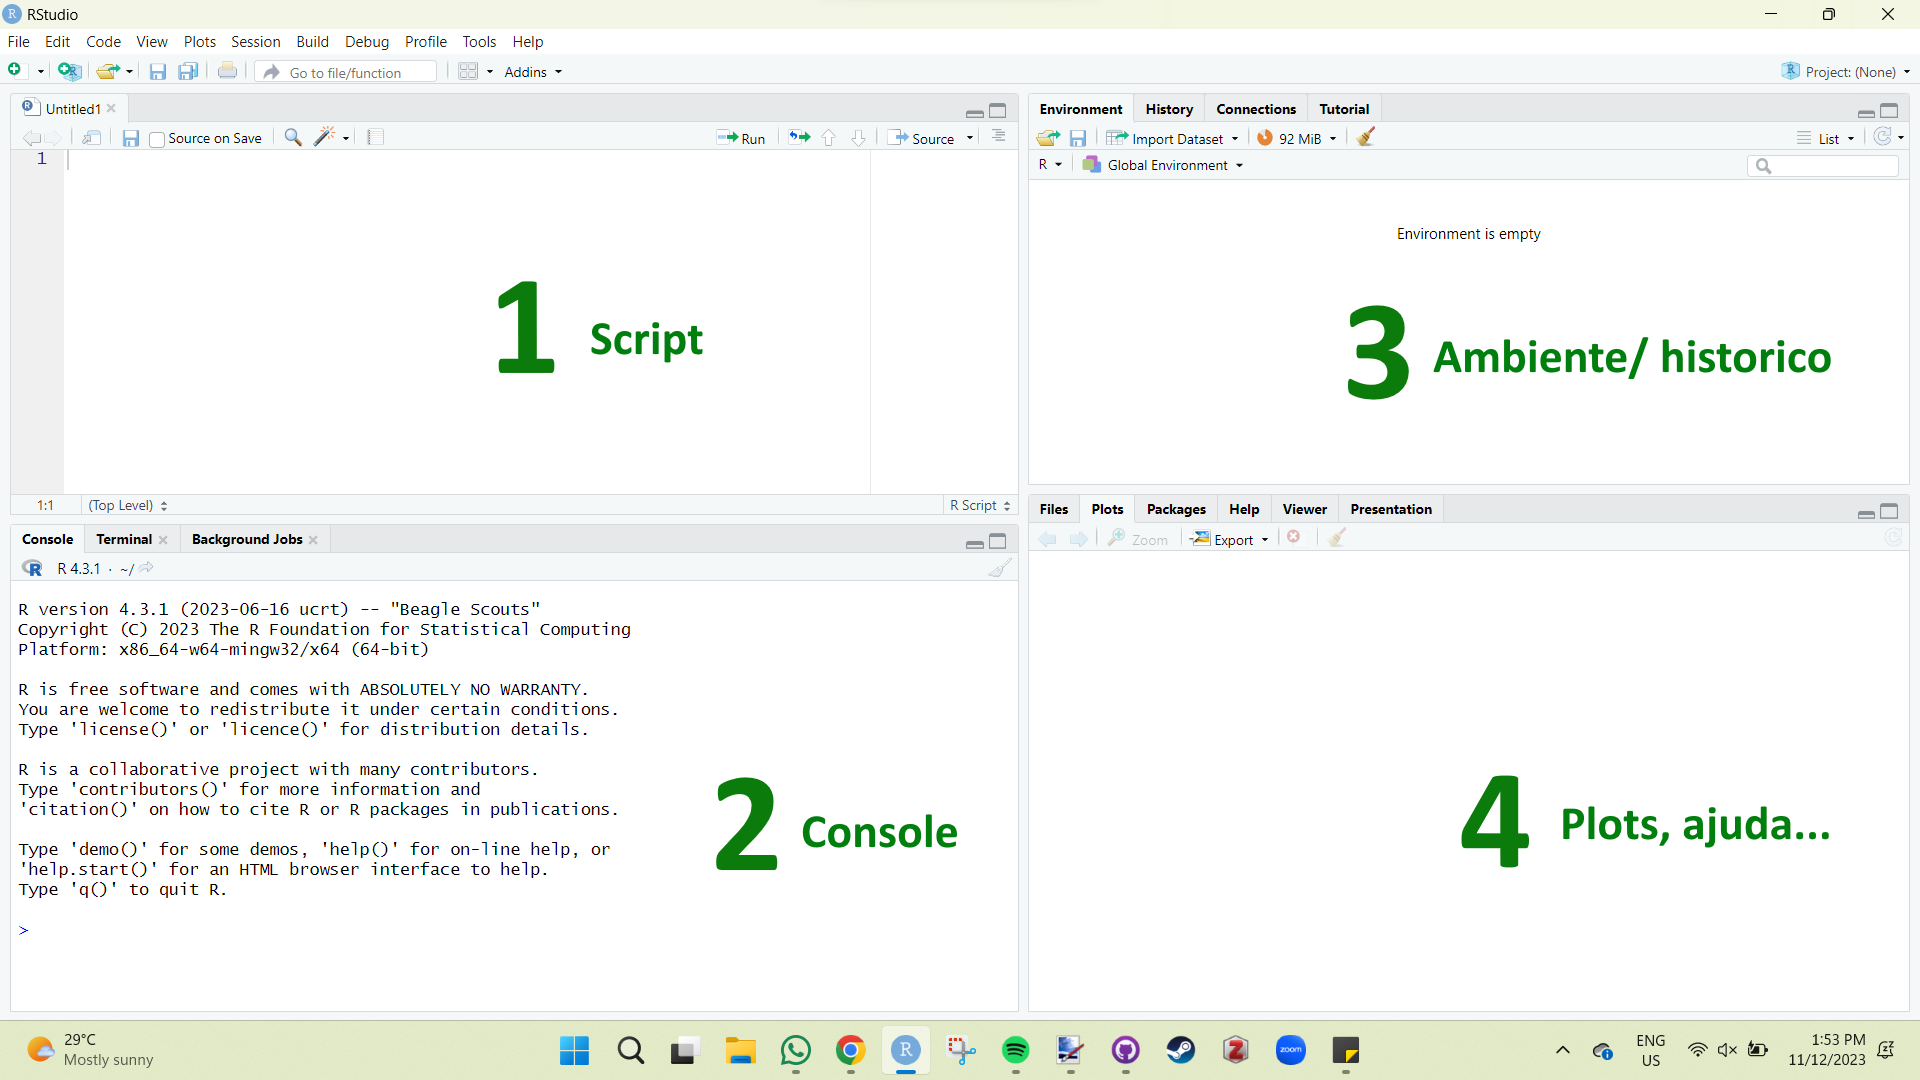
\includegraphics{img/cara_do_rstudio1.png}

Não tem a aparência convencional dos programas estatísticos, mas isso acontece porque não se realizam tarefas clicando em abas ou botões. No R Studio, você executa comandos por meio de códigos! No futuro, é provável que exista um programa com o qual você poderá conversar em qualquer idioma e ele realizará as tarefas que você pedir. Nao, pera, isso ja existe! Se chama inteligencia artificial! Entretanto, nao se deixe enganar. Os conhecimentos intimos de como pensar, organizar, analisar e mostrar seus dados sao importantissimos para todo um projeto cientifico. Mas se isso nao te convence, as melhores inteligencias artificiais do mercado sao pagas e podem te retornar resultados enganosos. Entao tenha muito cuidado e utilize as inteligencias artificiais disponiveis apenas como uma ferramenta auxiliar!

Vamos ao que importa e entender como o R funciona. O R possui uma linguagem, e tudo que voce vai fazer no R eh utilizando essa linguagem que sao verdadeiros comandos. Importe essa planilha! Crie esse grafico! Faca a media dessa variavel! E por ai vai. Entao vamos dar o nosso primeiro comando para o R e falar diretamente com ele. Pediremos que ele some 1 + 1, e para fazer isso iremos digitar 1 + 1 no console (Figura 2 - janela 2) e apertar a tecla ``Enter''.

\begin{Shaded}
\begin{Highlighting}[]
\DecValTok{1}\SpecialCharTok{+}\DecValTok{1}
\end{Highlighting}
\end{Shaded}

Ao fazer isso, ele vai te retornar o valor 2. Voce pode utilizar o R como uma calculadora e e realizar as operacoes basicas normalmente. Agora vamos pedir para ele diminuir 10 - 5, digitando no console e dando enter. Perceba que nao faz diferenca se voce digitar 10-5, 10 - 5, 10-5, ou ate mesmo 10 -5. Mas claro que ao escrever codigos iremos utilizar a forma que mantem o codigo mais organizado. Minha sugestao eh utilizar 10 - 5.

\begin{Shaded}
\begin{Highlighting}[]
\DecValTok{10} \SpecialCharTok{{-}} \DecValTok{5}
\end{Highlighting}
\end{Shaded}

Agora vamos pedir para ele multiplicar:

\begin{Shaded}
\begin{Highlighting}[]
\DecValTok{5} \SpecialCharTok{*} \DecValTok{5}
\end{Highlighting}
\end{Shaded}

E dividir:

\begin{Shaded}
\begin{Highlighting}[]
\DecValTok{10} \SpecialCharTok{/} \DecValTok{2}
\end{Highlighting}
\end{Shaded}

Voce pode encontrar como realizar potenciacao, raiz quadrada, entre outras coisas pesquisando facilmente na internet. Essa eh uma das vantagens do R. Ser gratuito, possuir codigo aberto, e uma comunidade altamente ativa, torna o R unico. Ao longo do livro voce encontrara alguns topicos onde eu peco para voce realizar pequenas tarefas para voce compreender o codigo e desenvolver autonomia.

\begin{itemize}
\tightlist
\item
  Pesquise como realizar potenciacao no R e calcule 2 elevado a 2.
  \emph{Dica: voce pode utilizar o chatgpt.}
\end{itemize}

Massa! Mas voce deve concordar comigo que essa forma de conversar com o R nao eh muito eficiente. Apesar de mostrar o historico, se voce quiser realizar a primeira operacao que fizemos (1 + 1), voce precisara digitar de novo, e de novo sempre que quiser fazer algo. Por esse motivo, a janela de script (Figura 2 - janela 1) se torna tao importante.

Vamos criar um script e utiliza-lo em uma situacao pratica. Mas antes precisamos aprender mais alguns botoes. Veja a figura abaixo:

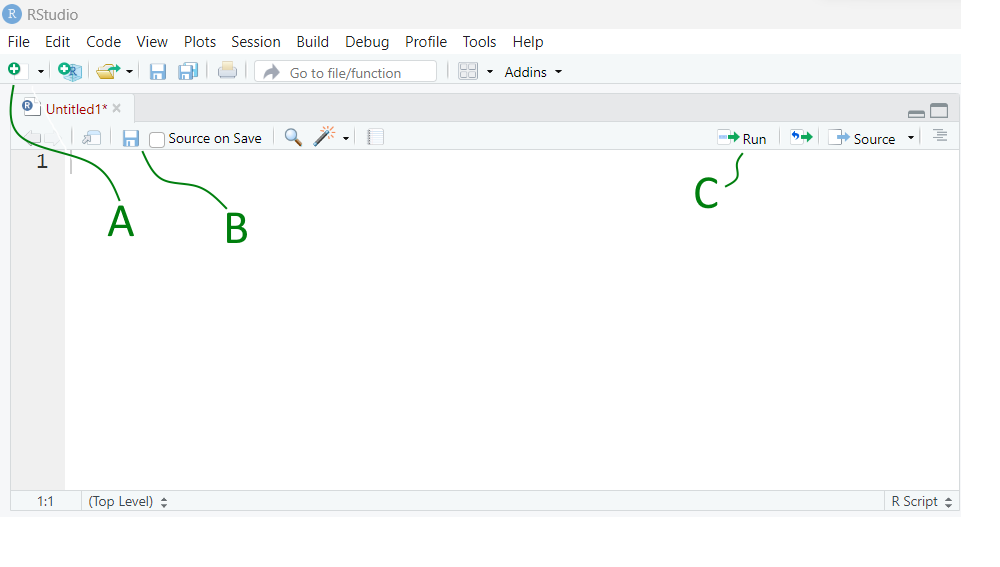
\includegraphics{img/Figura3_script.png}
Vamos criar um novo Script clicando no \textbf{botao ``A'' \textgreater{} New Script}. No Script, podemos digitar livremente sem que o codigo seja executado, inclusive podemos fazer comentarios utilizando o simbolo \textbf{\#} antes do que foi digitado. Podemos dar enter sem enviar o codigo para o R. O codigo apenas sera executado se clicarmos na linha do codigo e apertarmos o botao ``C'' (Run) ou \textbf{Ctrl + Enter}. Copie e cole o codigo abaixo no seu script e execute apertando Ctrl + Enter linha por linha. Perceba que a \# impede do nome Script ser executado. Se voce executar Script sem a \# o R nao vai entender e vai dar erro.

\begin{Shaded}
\begin{Highlighting}[]
\CommentTok{\#Script}

\DecValTok{1} \SpecialCharTok{+} \DecValTok{1}
\DecValTok{2}\SpecialCharTok{+} \DecValTok{2}
\DecValTok{10}\SpecialCharTok{/}\DecValTok{2}
\DecValTok{5}\SpecialCharTok{+}\DecValTok{5{-}2}\SpecialCharTok{/}\DecValTok{2}

\CommentTok{\#Fim}
\end{Highlighting}
\end{Shaded}

O comentario tambem pode ser feito na mesma linha depois do codigo, e assim, utilizar comentarios para explicar o que o codigo faz.

\begin{verbatim}
2*50 #Esse codigo realiza uma multiplicacao.
\end{verbatim}

Por fim, voce pode salvar o Script para acessa-lo sempre que quiser clicando no \textbf{botao ``B''} e selecionando um local no computador.

\hypertarget{objetos-vetores-e-funuxe7uxf5es}{%
\section{Objetos, vetores e funções}\label{objetos-vetores-e-funuxe7uxf5es}}

\hypertarget{objetos}{%
\subsection{Objetos}\label{objetos}}

Uma das funcoes mais importantes do R eh a capacidade de armazenar valores em objetos. Por exemplo, podemos dizer que o numero 1 sera atribuido a letra \textbf{``a''}, e para isso utilizamos o sinal de igual (=). O ``\textbf{a}'' agora eh considerado um objeto e ira aparecer na janela de Environment (Figura 2 - janela 3).

\begin{Shaded}
\begin{Highlighting}[]
\CommentTok{\# Mini Script  }
\NormalTok{a }\OtherTok{=} \DecValTok{1}  
\NormalTok{b }\OtherTok{=} \DecValTok{2}  
\end{Highlighting}
\end{Shaded}

Entretanto, o sinal de atribuicao mais utilizado eh a setinha (\textless-), devido a sua direcionalidade. Entao vamos adotar esse simbolo de atribuicao. Entao guarde isso na sua cabecinha: o codigo \textbf{\textless-} significa \textbf{atribuir}.

\begin{Shaded}
\begin{Highlighting}[]
\NormalTok{c }\OtherTok{\textless{}{-}} \DecValTok{3} \CommentTok{\# c recebe 3}
\NormalTok{d }\OtherTok{\textless{}{-}} \DecValTok{5} \CommentTok{\# atribuimos 5 ao d}
\end{Highlighting}
\end{Shaded}

Se voce esta copiando e colocando os codigos do livro no seu script, e apertando \textbf{Ctrl + Enter} em cada linha. Voce criou quatro objetos atraves das atribuicoes. Objetos a, b, c, d.~Mas voce so recebera o seu respectivo valor se voce digitar o objeto e executa-lo com Ctrl + Enter.

\begin{Shaded}
\begin{Highlighting}[]
\NormalTok{a}
\NormalTok{b}
\NormalTok{c}
\NormalTok{d}
\end{Highlighting}
\end{Shaded}

Com esses objetos podemos realizar operacoes matematicas.

\begin{Shaded}
\begin{Highlighting}[]
\CommentTok{\#Operacoes com objetos}

\NormalTok{a }\SpecialCharTok{+}\NormalTok{ b}
\NormalTok{c }\SpecialCharTok{*}\NormalTok{ d}
\NormalTok{b}\SpecialCharTok{/}\DecValTok{2}
\DecValTok{2} \SpecialCharTok{*}\NormalTok{ d}

\CommentTok{\#Fim}
\end{Highlighting}
\end{Shaded}

\emph{Nesse momento, nobre leitor, eu espero que voce esteja realizando diferentes operacoes matematicas, utilizando diferentes atribuicoes.}

Podemos atribuir valores em palavras inteiras. Como por exemplo, atribuir 10 ao objeto chamado ``nota'' (ou qualquer outra palavra).

\begin{Shaded}
\begin{Highlighting}[]
\NormalTok{nota }\OtherTok{\textless{}{-}} \DecValTok{10}
\NormalTok{Nota }\OtherTok{\textless{}{-}} \DecValTok{0}
\end{Highlighting}
\end{Shaded}

Perceba que o R detecta as diferencas entre letras maiusculas e minusculas. Portanto, ``nota'' eh diferente de ``Nota''. Muito cuidado com isso. Para evitar erros, sugiro sempre utilizar letras minusculas.

Alguns simbolos nao podem ser utilizados para criar objetos, uma vez que eles sao reservados no R. Como por exemplo o ``-'', ou TRUE / FALSE. Perceba que ao rodar os codigos abaixo, o R ira retornar um erro.

\begin{Shaded}
\begin{Highlighting}[]
\ConstantTok{FALSE} \OtherTok{\textless{}{-}} \DecValTok{2}
\ConstantTok{TRUE} \OtherTok{\textless{}{-}} \DecValTok{5}
\NormalTok{guarda}\SpecialCharTok{{-}}\NormalTok{chuva }\OtherTok{\textless{}{-}} \DecValTok{2}
\end{Highlighting}
\end{Shaded}

Tambem podemos atribuir uma equacao inteira a um objeto. Na verdade podemos atribuir quase tudo a um objeto, graficos, resultados, planilhas, etc. Mas isso veremos mais a frente.

\begin{Shaded}
\begin{Highlighting}[]
\CommentTok{\#Note que o underline (\_) funciona bem para separar palavras, assim como ponto (.)}
\NormalTok{guarda\_chuva }\OtherTok{\textless{}{-}} \DecValTok{2}\SpecialCharTok{*}\DecValTok{10}\SpecialCharTok{/}\DecValTok{2}
\NormalTok{guarda\_chuva}

\NormalTok{guarda.roupa }\OtherTok{\textless{}{-}} \DecValTok{2}\SpecialCharTok{*}\DecValTok{100}\SpecialCharTok{/}\DecValTok{10}
\NormalTok{guarda.roupa}
\end{Highlighting}
\end{Shaded}

Alem disso tudo, podemos atribuir um texto a um objeto. Mas para isso o texto precisa estar entre aspas.

\begin{Shaded}
\begin{Highlighting}[]
\CommentTok{\#Atribuindo a palavra "coxinha" ao objeto melhor\_comida}
\NormalTok{melhor\_comida }\OtherTok{\textless{}{-}} \StringTok{"coxinha"}
\NormalTok{melhor\_comida}
\end{Highlighting}
\end{Shaded}

Mas para o que serve tudo isso? Para que aprender essas coisas? A resposta principal eh a capacidade de automatizacao e reprodutibilidade das suas analises.

Vamos criar um exemplo pratico para fixar conceitos. Vamos imaginar que queremos calcular quanto gastamos de aluguel por mes e ano, considerando que pagamos o aluguel semanalmente. Vamos supor que o aluguel por semana seja 200 reais.

\begin{Shaded}
\begin{Highlighting}[]
\CommentTok{\#Calculando o aluguel}

\NormalTok{aluguel\_semana }\OtherTok{\textless{}{-}} \DecValTok{200}              \CommentTok{\#valor do aluguel por semana}
\NormalTok{aluguel\_mes }\OtherTok{\textless{}{-}} \DecValTok{4} \SpecialCharTok{*}\NormalTok{ aluguel\_semana  }\CommentTok{\#considerando que 1 mes possui 4 semanas.}
\NormalTok{aluguel\_ano }\OtherTok{\textless{}{-}} \DecValTok{12} \SpecialCharTok{*}\NormalTok{ aluguel\_mes    }\CommentTok{\#o ano possui 12 meses eh serio}

\NormalTok{aluguel\_semana}
\NormalTok{aluguel\_mes}
\NormalTok{aluguel\_ano}
\end{Highlighting}
\end{Shaded}

Veja que massa! Criamos um script para calcular o valor do aluguel por mes e ano. Com esse script, voce pode calcular facilmente diferentes situacoes, simulando diferentes valores de aluguel. Para isso, eh so alterar o valor 200 de aluguel\_semana para o valor desejado e rodar linha por linha.

\begin{itemize}
\tightlist
\item
  \emph{Substititua ``aluguel\_semana \textless- 200'' por ``aluguel\_semana \textless- 247.53}''
\end{itemize}

Se voce pode fazer isso para calcular o aluguel, imagina o que esse sistema pode fazer com sua analise de dados.

\hypertarget{vetores}{%
\subsection{Vetores}\label{vetores}}

Os objetos com multiplos valores de um mesmo tipo sao chamados de vetores. Para criar um objeto vetor inserimos os valores dentro de parenteses separados por virgulas. Virgulas no R servem para separar o codigo. Entao se voce quiser digitar numeros quebrados nunca utilize \textbf{virgula}, utilize \textbf{ponto}.

\begin{Shaded}
\begin{Highlighting}[]
\NormalTok{vetor.A }\OtherTok{\textless{}{-}} \FunctionTok{c}\NormalTok{(}\FloatTok{10.5}\NormalTok{, }\FloatTok{20.6}\NormalTok{, }\FloatTok{30.2}\NormalTok{)}
\NormalTok{vetor.B }\OtherTok{\textless{}{-}} \FunctionTok{c}\NormalTok{(}\DecValTok{2}\NormalTok{, }\DecValTok{2}\NormalTok{, }\DecValTok{2}\NormalTok{)}
\NormalTok{melhores.comidas }\OtherTok{\textless{}{-}} \FunctionTok{c}\NormalTok{(}\StringTok{"coxinha"}\NormalTok{,}\StringTok{"pastel"}\NormalTok{,}\StringTok{"lasanha"}\NormalTok{) }\CommentTok{\#Lembre{-}se, caracteres precisam estar dentro de aspas.}

\NormalTok{vetor.A}
\NormalTok{vetor.B}
\NormalTok{melhores.comidas}
\end{Highlighting}
\end{Shaded}

\hypertarget{funuxe7uxf5es}{%
\subsection{Funções}\label{funuxe7uxf5es}}

No R, as funcoes servem para processar de alguma forma os dados. O R ja possui algumas funcoes nativas, como por exemplo para calcular a raiz quadrada de um numero. A funcao possui um nome, geralmente associado ao que ela faz, e argumentos que eh o tipo de dado que voce precisa inserir nela para ser calculado. Vamos dar uma olhada na funcao \emph{sqrt()}. A sigla ``sqrt'' representa ``square root'' em ingles. Primeiro vamos rodar a funcao sem argumentos, apenas o \emph{sqrt()} e depois inserimos o argumento, que nesse caso, eh um numero.

\begin{Shaded}
\begin{Highlighting}[]
\CommentTok{\#funcao que calcula raiz quadrada}

\FunctionTok{sqrt}\NormalTok{()}

\FunctionTok{sqrt}\NormalTok{(}\DecValTok{25}\NormalTok{)}
\end{Highlighting}
\end{Shaded}

Note que quando nao colocamos (ou erramos) o argumento, a R vai te retornar um erro, geralmente, explicando o problema.

Existem funcoes dentro do R para todo tipo de coisa! Vamos criar um conjunto de dados e fazer alguns calculos utilizando algumas funcoes.

\begin{Shaded}
\begin{Highlighting}[]
\CommentTok{\#Notas do terceiro ano A}
\NormalTok{notas }\OtherTok{\textless{}{-}} \FunctionTok{c}\NormalTok{(}\DecValTok{7}\NormalTok{, }\DecValTok{8}\NormalTok{, }\DecValTok{10}\NormalTok{, }\DecValTok{5}\NormalTok{, }\DecValTok{2}\NormalTok{, }\DecValTok{4}\NormalTok{, }\FloatTok{6.6}\NormalTok{, }\FloatTok{7.9}\NormalTok{, }\FloatTok{8.9}\NormalTok{, }\DecValTok{0}\NormalTok{)}

\CommentTok{\#Qual a media da turma?}
\FunctionTok{mean}\NormalTok{(notas)}

\CommentTok{\#Qual a mediana?}
\FunctionTok{median}\NormalTok{(notas)}

\CommentTok{\#Qual o desvio padrao das notas?}
\FunctionTok{sd}\NormalTok{(notas)}

\CommentTok{\#Qual a menor e a maior nota?}
\FunctionTok{min}\NormalTok{(notas)}
\FunctionTok{max}\NormalTok{(notas)}

\CommentTok{\#resumo das notas}
\FunctionTok{summary}\NormalTok{(notas)}
\end{Highlighting}
\end{Shaded}

Cada uma dessas funcoes realiza algum calculo em especifico, no caso de \emph{summary()}, ela realiza o calculo da media, mediana, maximo, minimo e quartis, tudo ao mesmo tempo. Talvez em algum momento voce nao encontre a funcao que voce precisa para determinada tarefa, nesse caso, voce pode criar sua propria funcao! Voce pode criar uma funcao utilizando outras funcoes, para fazer algo especifico para voce. Por enquanto, vamos apenas ser usuario de funcoes e nao criadores. Mas se voce realmente quer saber como criar uma funcao, nao irei te limitar. Abaixo voce encontra um dos exemplos mais simples de funcao. Utilize sua criatividade, seus conhecimentos de objetos, funcoes e vetores para criar alguma funcao. Mas sinta-se a vontade para pular essa parte, uma vez que ela nao eh essencial ao uso do R.

\hypertarget{criando-uma-funcao-opcional}{%
\subsubsection{Criando uma funcao (opcional)}\label{criando-uma-funcao-opcional}}

Vamos imaginar que voce precise criar uma funcao para somar dois numeros. Uma funcao simples mas que vai nos ajudar a entender a estrutura de uma funcao. Para criar uma funcao, precisamos utilizar a funcao chamada de \emph{function()}.

\begin{Shaded}
\begin{Highlighting}[]
\CommentTok{\#Estrutura de uma funcao:}

\NormalTok{nome\_da\_funcao }\OtherTok{\textless{}{-}} \ControlFlowTok{function}\NormalTok{() \{ \}}

\CommentTok{\#Criando a funcao soma}

\NormalTok{soma }\OtherTok{\textless{}{-}} \ControlFlowTok{function}\NormalTok{(n1, n2) \{}

\NormalTok{add }\OtherTok{\textless{}{-}}\NormalTok{ n1 }\SpecialCharTok{+}\NormalTok{ n2}
\FunctionTok{print}\NormalTok{(add)}

\NormalTok{\}}
\end{Highlighting}
\end{Shaded}

Essa eh uma funcao que possui dois argumentos (n1, n2) e utilizando esses argumentos ela realiza um calculo de soma e atribui esse resultado a um objeto que chamamos de ``add''. Por fim, utilizamos a funcao \emph{print()} para mostrar o valor embutido em ``add''.

Agora, vamos imaginar que talvez a funcao \emph{summary()} nao seja o que voce precisa. Voce precisa mesmo eh de uma funcao que te forneca, media, mediana e desvio padrao dos seus dados.

Nesse caso, podemos criar a funcao \emph{my\_summary()} utilizando a funcao \emph{function()}.

\begin{Shaded}
\begin{Highlighting}[]
\CommentTok{\#Criando a funcao my\_summary()}

\NormalTok{my\_summary }\OtherTok{\textless{}{-}} \ControlFlowTok{function}\NormalTok{(v) \{}

\NormalTok{media   }\OtherTok{\textless{}{-}} \FunctionTok{mean}\NormalTok{(v)}
\NormalTok{mediana }\OtherTok{\textless{}{-}} \FunctionTok{median}\NormalTok{(v)}
\NormalTok{desvio  }\OtherTok{\textless{}{-}} \FunctionTok{sd}\NormalTok{(v)}

\NormalTok{resultado }\OtherTok{\textless{}{-}} \FunctionTok{c}\NormalTok{(media, mediana, desvio)}
\FunctionTok{print}\NormalTok{(resultado)}

\NormalTok{\}}
\end{Highlighting}
\end{Shaded}

Calma, tem muita coisa ai, mas eh tudo o que a gente ja sabe. Na funcao \emph{my\_summary()}, precisamos inserir apenas um argumento do tipo vetor, como por exemplo, nosso objeto ``notas''. Esse argumento sera aplicado a tudo que possuir o caractere ``v'' dentro da funcao. O ``v'' a gente definiu em function(v). Mais uma vez, as chaves \textbf{\{\}} que abre e fecha contem tudo o que a gente quer que a funcao realize, linha por linha. Primeiro, queremos que a nossa funcao calcule a media e atribua o resultado a um objeto chamado ``media''. Segundo, calcular a mediana e atribuir o resultado a um objeto chamado ``mediana'', depois o desvio. Depois criamos um vetor chamado de ``resultado'' que armazena os objetos ``media'', ``mediana'' e ``desvio''. Em seguida, pedimos para o R nos mostrar os valores desse vetor ``resultado'' utilizando a funcao \emph{print()}.

Vamos usar nossa funcao personalizada para calcular nosso objeto ``notas''.

\begin{Shaded}
\begin{Highlighting}[]
\CommentTok{\#Notas do terceiro ano A}
\NormalTok{notas }\OtherTok{\textless{}{-}} \FunctionTok{c}\NormalTok{(}\DecValTok{7}\NormalTok{, }\DecValTok{8}\NormalTok{, }\DecValTok{10}\NormalTok{, }\DecValTok{5}\NormalTok{, }\DecValTok{2}\NormalTok{, }\DecValTok{4}\NormalTok{, }\FloatTok{6.6}\NormalTok{, }\FloatTok{7.9}\NormalTok{, }\FloatTok{8.9}\NormalTok{, }\DecValTok{0}\NormalTok{)}

\CommentTok{\#Utilizando a funcao my\_summary()}

\FunctionTok{my\_summary}\NormalTok{(notas)}
\end{Highlighting}
\end{Shaded}

Veja que a funcao retornou os valores do nosso vetor, mas apenas isso. Mais para frente, a gente ve como criar funcoes mais elaboradas, como por exemplo para simular gastos de alugueis como anteriormente.

\hypertarget{tabela-de-dados}{%
\section{Tabela de dados}\label{tabela-de-dados}}

\hypertarget{data-frame}{%
\subsection{Data frame}\label{data-frame}}

Data frame nada mais eh do que uma tabela de dados. Vamos direto ao que interessa e usar a funcao \emph{data.frame()} para criar uma tabela. Iremos criar as notas de 10 alunos e seus respectivos nomes. Se voce ainda estiver na mesma sessao de R, podemos ver que o objeto ``notas'' ainda esta salvo na janela 3 (Environment e History) e podemos aproveita-lo. De qualquer forma vou recriar ``notas'', caso por algum motivo voce SAIU do R, um absurdo, mas acontece.

\begin{Shaded}
\begin{Highlighting}[]
\CommentTok{\#Criando um data frame contendo as notas e os nomes de cada aluno}

\CommentTok{\#Primeiro criamos as notas}
\NormalTok{notas }\OtherTok{\textless{}{-}} \FunctionTok{c}\NormalTok{(}\DecValTok{7}\NormalTok{, }\DecValTok{8}\NormalTok{, }\DecValTok{10}\NormalTok{, }\DecValTok{5}\NormalTok{, }\DecValTok{2}\NormalTok{, }\DecValTok{4}\NormalTok{, }\FloatTok{6.6}\NormalTok{, }\FloatTok{7.9}\NormalTok{, }\FloatTok{8.9}\NormalTok{, }\DecValTok{0}\NormalTok{) }

\CommentTok{\#Segundo criamos os nomes}
\NormalTok{nomes }\OtherTok{\textless{}{-}} \FunctionTok{c}\NormalTok{(}\StringTok{"Marilia"}\NormalTok{, }\StringTok{"Jonatas"}\NormalTok{, }\StringTok{"Guilherme"}\NormalTok{, }\StringTok{"Camila"}\NormalTok{, }
\StringTok{"Fiuza"}\NormalTok{, }\StringTok{"Brunno"}\NormalTok{, }\StringTok{"Diego"}\NormalTok{, }\StringTok{"Mathews"}\NormalTok{, }\StringTok{"Biny"}\NormalTok{, }\StringTok{"Rebecca"}\NormalTok{)}

\CommentTok{\#Terceiro utilizamos a funcao data.frame() para criar a tabela}
\NormalTok{tabela }\OtherTok{\textless{}{-}} \FunctionTok{data.frame}\NormalTok{(nomes, notas)}
\NormalTok{tabela}
\end{Highlighting}
\end{Shaded}

Esse data.frame (tabela), eh uma forma muito simplificada das tabelas que iremos importar de nossos dados reais. Porem, ela nos serve muito bem para entendermos como funciona uma planilha no R.

A partir de agora eu quero que voce perceba uma coisa muito importante e leve isso para a vida. Uma planilha organizada deve ser construida da seguinte forma:

-Variaveis sao colunas;
-Observacoes sao linhas;
-Cada valor na sua celula.

Com essa formatacao de planilha, voce consegue fazer quase tudo no R, para manipulacao de dados, construcao de graficos e analises estatisticas.

Logo, para voce acessar uma variavel de uma tabela, voce pode usar o \textbf{\$} da seguinte forma:

\begin{Shaded}
\begin{Highlighting}[]
\CommentTok{\#Acessando uma variavel}

\NormalTok{tabela}\SpecialCharTok{$}\NormalTok{nomes}
\NormalTok{tabela}\SpecialCharTok{$}\NormalTok{notas}
\end{Highlighting}
\end{Shaded}

Perceba que quando voce digita \textbf{tabela\$} voce pode apertar a tecla TAB para mostrar e selecionar as variaveis de sua tabela. Caso alguma nota esteja errada e voce queira corrigi-la, voce pode utilizar a funcao \emph{fix()}. Essa funcao abre uma janela onde voce pode clicar e modificar o valor desejado.

\begin{Shaded}
\begin{Highlighting}[]

\FunctionTok{fix}\NormalTok{(tabela)}
\end{Highlighting}
\end{Shaded}

Quse nunca utilizamos a funcao \emph{fix()} para corrigir os dados, mas eh interessante saber que o R pode abrir novas janelas e criar coisas interativas.

Agora sabendo como acessar as variaveis de uma tabela, voce pode utilizar funcoes para calcular uma variavel especifica do data frame.

\begin{Shaded}
\begin{Highlighting}[]
\FunctionTok{mean}\NormalTok{(tabela}\SpecialCharTok{$}\NormalTok{notas)}
\end{Highlighting}
\end{Shaded}

Utilize as funcoes abaixo para calcular mediana, maximo, minimo:

\begin{itemize}
\tightlist
\item
  median()
\item
  max()
\item
  min()
\item
  summary()
\end{itemize}

\hypertarget{planilha-de-dados-nativa-do-r}{%
\subsection{Planilha de dados nativa do R}\label{planilha-de-dados-nativa-do-r}}

O R possui um banco de dados que nos fornece algumas tabelas de estudo reais o quais podemos utilizar para treinar nossas habilidades. Para isso, precisamos dizer para o R qual banco de dados queremos invocar utilizando a funcao \emph{data()}.

\begin{Shaded}
\begin{Highlighting}[]
\CommentTok{\#Importando o banco de dados "iris" do R}
\FunctionTok{data}\NormalTok{(iris)}

\CommentTok{\#Funcoes exploratorias}
\FunctionTok{head}\NormalTok{(iris) }\CommentTok{\#Mostra a parte de cima da planilha }
\FunctionTok{tail}\NormalTok{(iris) }\CommentTok{\#Mostra a parte de baixo}
\FunctionTok{str}\NormalTok{(iris)  }\CommentTok{\#Mostra os tipos das variaveis}
\end{Highlighting}
\end{Shaded}

Veja que ao usarmos a funcao \emph{str()} o R retorna a natureza das variaveis da planilha.

\begin{itemize}
\tightlist
\item
  \emph{num} significa numerica.
\item
  \emph{Factor} significa que eh uma variavel qualitativa com fatores (setosa, versicolor, virginica).
\end{itemize}

As vezes a planilha eh importada com as variaveis mal formatadas e isso pode gerar problemas de reconhecimento por parte do R. Nesse caso, eh sempre interessante realizar a verificacao dos dados utilizando a funcao \emph{str()} ou outras funcoes similares. Caso o R nao esteja identificando as variaveis corretamente, duas funcoes muito uteis podem ser utilizadas: \emph{as.numeric()} e \emph{as.factor()}.

\begin{Shaded}
\begin{Highlighting}[]
\FunctionTok{data}\NormalTok{(iris)}

\CommentTok{\#Convertendo variavel para numerica}
\NormalTok{iris}\SpecialCharTok{$}\NormalTok{Sepal.Length }\OtherTok{\textless{}{-}} \FunctionTok{as.numeric}\NormalTok{(iris}\SpecialCharTok{$}\NormalTok{Sepal.Length)}

\CommentTok{\#Convertendo variavel para fator}
\NormalTok{iris}\SpecialCharTok{$}\NormalTok{Species }\OtherTok{\textless{}{-}} \FunctionTok{as.factor}\NormalTok{(iris}\SpecialCharTok{$}\NormalTok{Species)}
\end{Highlighting}
\end{Shaded}

Basicamente voce ta transformando em numerica a variavel Sepal length da planilha iris e atribuindo a ela mesma. Dessa forma, voce faz a alteracao de forma permanente. A mesma coisa ocorre com as.factor.

Vamos brincar um pouco com a planilha iris. Primeiro veja que ela esta construida de forma organizada (variaveis nas colunas, observacoes nas linhas, cada celula um valor). Podemos entao realizar o summary() para saber a media, mediana, maximo e minimo da largura da petala (Petal.Width).

\begin{Shaded}
\begin{Highlighting}[]
\FunctionTok{summary}\NormalTok{(iris}\SpecialCharTok{$}\NormalTok{Petal.Width)}
\end{Highlighting}
\end{Shaded}

Porem note que existe 3 especies diferentes. A funcao \emph{summary()} nao leva isso em consideracao. O ideal seria calcular o \emph{summary()} para cada especie. Para isso temos uma funcao muito legal chamada \emph{tapply()}, onde: o primeiro argumento eh a variavel numerica, o segundo a variavel com os fatores, e o terceiro argumento eh a funcao que voce quer aplicar.

\begin{Shaded}
\begin{Highlighting}[]
\FunctionTok{tapply}\NormalTok{(iris}\SpecialCharTok{$}\NormalTok{Petal.Width, iris}\SpecialCharTok{$}\NormalTok{Species, summary)}
\end{Highlighting}
\end{Shaded}

\hypertarget{importando-sua-planilha}{%
\subsection{Importando sua planilha}\label{importando-sua-planilha}}

No RStudio podemos importar uma planilha do formato excel (xlsx) utilizando o botao na janela Environment (superior direita):

Environment \textgreater{} Import Dataset \textgreater{} From excel

Acho pouco eficiente ensinar a importar dados de um diretorio. Acho pouco pratico, uma vez que temos o botao de importar. Ao inves disso, irei treina-lo a utilizar projetos de R reprodutiveis e organizados. Ao trabalhar no R, voce seguira um protocolo basico de como tratar os dados a serem analisados. Ao longo do tempo, voce sera capaz de otimizar esse protocolo e aplicar para quase todo tipo de dado que voce possuir. De qualquer forma, saiba que o R trabalha com uma pasta especifica chamada de diretorio, e para saber qual eh o seu diretorio padrao, utilize a funcao \emph{getwd()}:

\begin{Shaded}
\begin{Highlighting}[]
\FunctionTok{getwd}\NormalTok{()}
\end{Highlighting}
\end{Shaded}

Ao executar esse funcao, o R te retornara o caminho da pasta do diretorio padrao atual que provavelmente eh a pasta ``documentos'' do seu computador.

Para baixar uma planilha de dados ficticios clique no link abaixo e tente importa-la atraves do botao \textbf{Import from excel}.

\href{data/fake_data.xlsx}{Clique aqui para baixar a planilha ficticia}

\hypertarget{graficos}{%
\section{Graficos}\label{graficos}}

Agora comeca a parte divertida! A visualizacao de dados no R tem um potencial quase infinito devido as sua grande capacidade de personalizar cada pedacinho da figura.

\hypertarget{grafico-de-histograma}{%
\subsection{Grafico de histograma}\label{grafico-de-histograma}}

Esse grafico nos mostra a frequencia dos valores da variavel de interesse, como por exemplo comprimento da petala das flores do banco de dados iris.

\begin{Shaded}
\begin{Highlighting}[]
\CommentTok{\#Importando banco de dados "iris"}
\FunctionTok{data}\NormalTok{(iris)}

\CommentTok{\#Criando histograma}
\FunctionTok{hist}\NormalTok{(iris}\SpecialCharTok{$}\NormalTok{Sepal.Length)}
\end{Highlighting}
\end{Shaded}

\begin{figure}
\centering
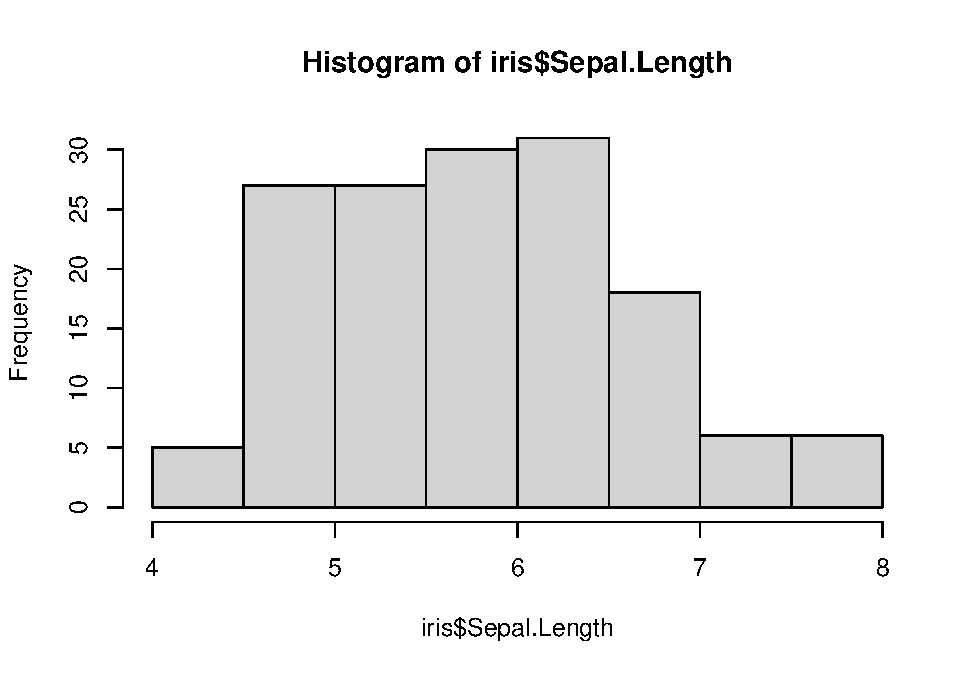
\includegraphics{_main_files/figure-latex/nome-do-chunk1-1.pdf}
\caption{\label{fig:nome-do-chunk1}Gráficos com R base}
\end{figure}

Simples nao eh? Mas podemos modificar ainda mais nosso grafico. Alterar cores, nomes dos eixos, titulo, etc. Vamos ver mais argumentos com o grafico de dispersao de pontos.

\hypertarget{grafico-de-dispersao}{%
\subsection{Grafico de dispersao}\label{grafico-de-dispersao}}

Esse grafico nos mostra a relacao entre duas variaveis continuas. Vamos utilizar o banco de dados ``iris'' para construir e visualizar alguns graficos. Para construir um grafico de dispersao utilizamos a funcao \emph{plot()}. Note que a funcao plot, possui varios argumentos que podemos ir adicionando para personalizar o grafico. Alem disso, para deixar o codigo mais organizado, sempre apos a virgula de um argumento, pulamos a linha, de forma que cada argumento fique numa linha.

\begin{Shaded}
\begin{Highlighting}[]
\CommentTok{\#Cria o grafico basico}
\FunctionTok{plot}\NormalTok{(iris}\SpecialCharTok{$}\NormalTok{Sepal.Width, iris}\SpecialCharTok{$}\NormalTok{Petal.Width)}
\end{Highlighting}
\end{Shaded}

\begin{figure}
\centering
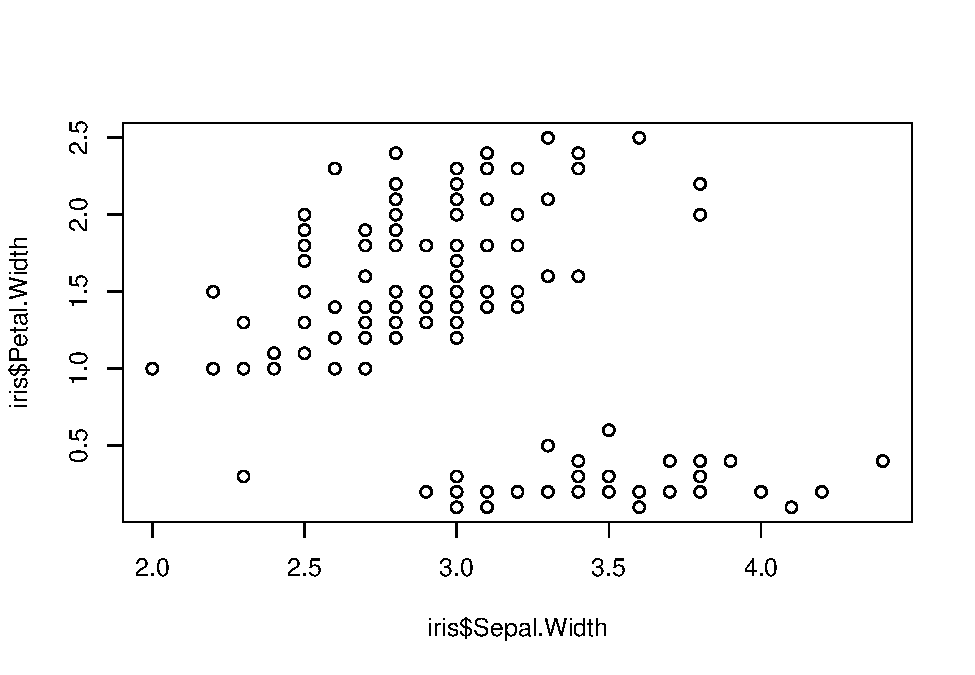
\includegraphics{_main_files/figure-latex/nome-do-chunk2-1.pdf}
\caption{\label{fig:nome-do-chunk2-1}Gráficos com R base}
\end{figure}

\begin{Shaded}
\begin{Highlighting}[]
\CommentTok{\#adiciona o argumento para mudar o nome do eixo y}
\FunctionTok{plot}\NormalTok{(iris}\SpecialCharTok{$}\NormalTok{Sepal.Width, iris}\SpecialCharTok{$}\NormalTok{Petal.Width, }
     \AttributeTok{ylab =} \StringTok{"Petal Width"}\NormalTok{)}
\end{Highlighting}
\end{Shaded}

\begin{figure}
\centering
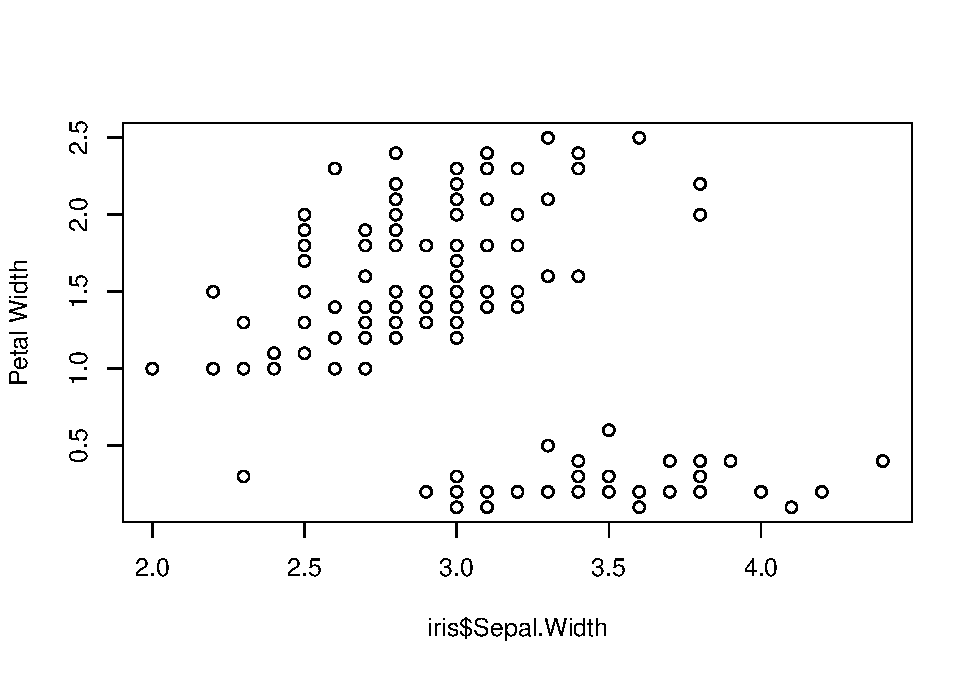
\includegraphics{_main_files/figure-latex/nome-do-chunk2-2.pdf}
\caption{\label{fig:nome-do-chunk2-2}Gráficos com R base}
\end{figure}

\begin{Shaded}
\begin{Highlighting}[]
\CommentTok{\#adiciona o argumento para mudar o nome do eixo x}
\FunctionTok{plot}\NormalTok{(iris}\SpecialCharTok{$}\NormalTok{Sepal.Width, iris}\SpecialCharTok{$}\NormalTok{Petal.Width, }
     \AttributeTok{ylab =} \StringTok{"Petal Width"}\NormalTok{, }
     \AttributeTok{xlab =} \StringTok{"Sepal Width"}
\NormalTok{     )}
\end{Highlighting}
\end{Shaded}

\begin{figure}
\centering
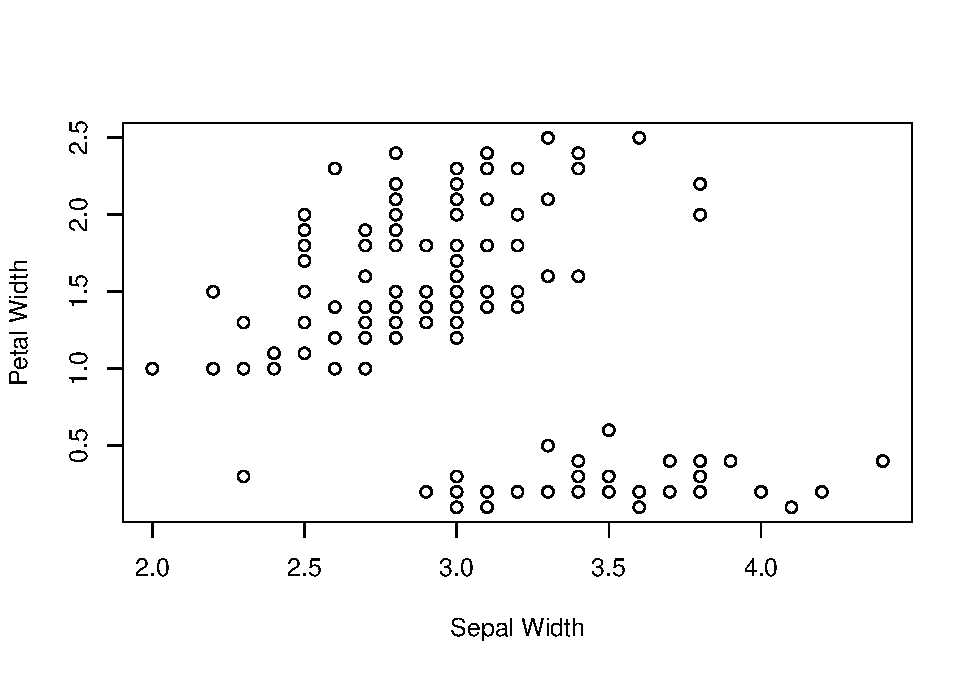
\includegraphics{_main_files/figure-latex/nome-do-chunk2-3.pdf}
\caption{\label{fig:nome-do-chunk2-3}Gráficos com R base}
\end{figure}

\begin{Shaded}
\begin{Highlighting}[]
\CommentTok{\#argumento para mudar a cor dos pontos}
\FunctionTok{plot}\NormalTok{(iris}\SpecialCharTok{$}\NormalTok{Sepal.Width, iris}\SpecialCharTok{$}\NormalTok{Petal.Width, }
     \AttributeTok{ylab =} \StringTok{"Petal Width"}\NormalTok{, }
     \AttributeTok{xlab =} \StringTok{"Sepal Width"}\NormalTok{,}
     \AttributeTok{col =} \StringTok{"blue"}
\NormalTok{     )}
\end{Highlighting}
\end{Shaded}

\begin{figure}
\centering
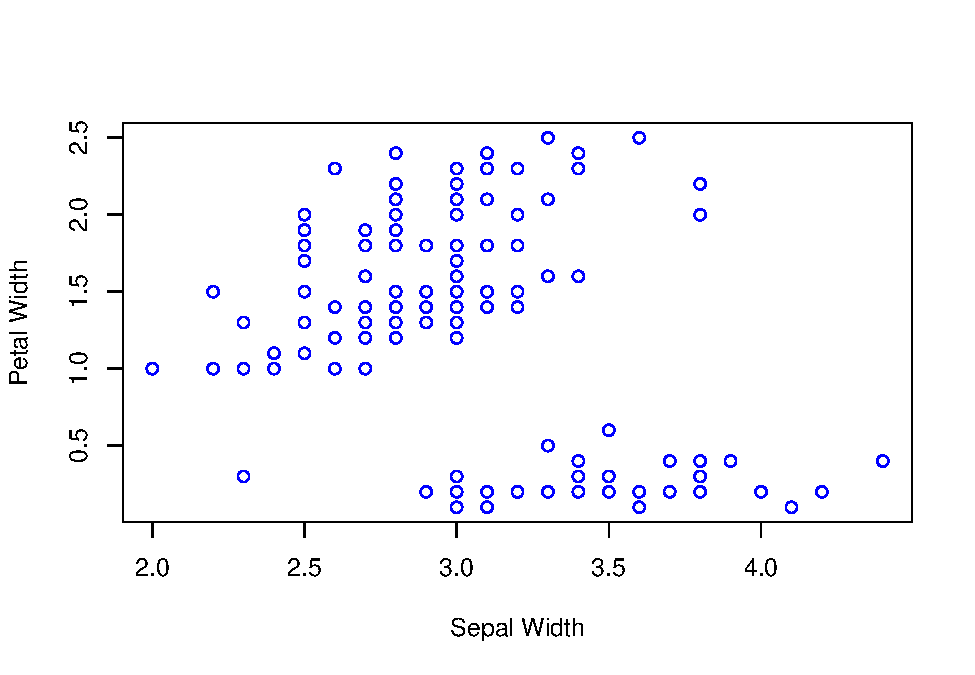
\includegraphics{_main_files/figure-latex/nome-do-chunk2-4.pdf}
\caption{\label{fig:nome-do-chunk2-4}Gráficos com R base}
\end{figure}

\begin{Shaded}
\begin{Highlighting}[]
\CommentTok{\#argumento para mudar o formato dos pontos}
\FunctionTok{plot}\NormalTok{(iris}\SpecialCharTok{$}\NormalTok{Sepal.Width, iris}\SpecialCharTok{$}\NormalTok{Petal.Width, }
     \AttributeTok{ylab =} \StringTok{"Petal Width"}\NormalTok{, }
     \AttributeTok{xlab =} \StringTok{"Sepal Width"}\NormalTok{,}
     \AttributeTok{col =} \DecValTok{3}\NormalTok{,}
     \AttributeTok{pch =} \DecValTok{2}
\NormalTok{     )}
\end{Highlighting}
\end{Shaded}

\begin{figure}
\centering
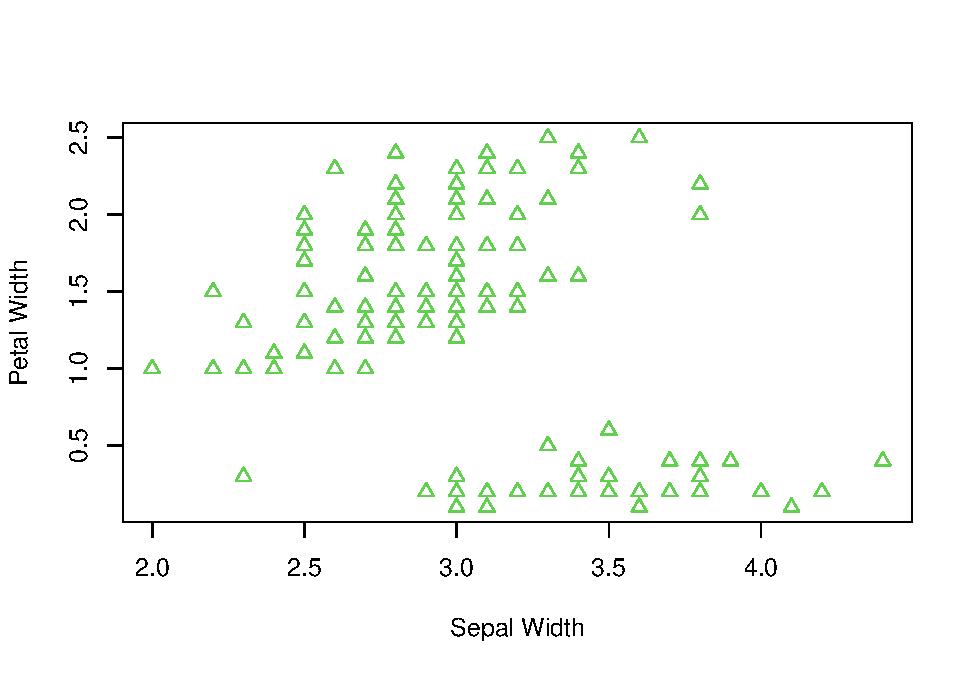
\includegraphics{_main_files/figure-latex/nome-do-chunk2-5.pdf}
\caption{\label{fig:nome-do-chunk2-5}Gráficos com R base}
\end{figure}

\begin{Shaded}
\begin{Highlighting}[]
\CommentTok{\#argumento para adicionar um titulo no grafico}
\FunctionTok{plot}\NormalTok{(iris}\SpecialCharTok{$}\NormalTok{Sepal.Width, iris}\SpecialCharTok{$}\NormalTok{Petal.Width, }
     \AttributeTok{ylab =} \StringTok{"Petal Width"}\NormalTok{, }
     \AttributeTok{xlab =} \StringTok{"Sepal Width"}\NormalTok{,}
     \AttributeTok{col =} \DecValTok{3}\NormalTok{,}
     \AttributeTok{pch =} \DecValTok{2}\NormalTok{,}
     \AttributeTok{main =} \StringTok{"Titulo do grafico"}
\NormalTok{     )}
\end{Highlighting}
\end{Shaded}

\begin{figure}
\centering
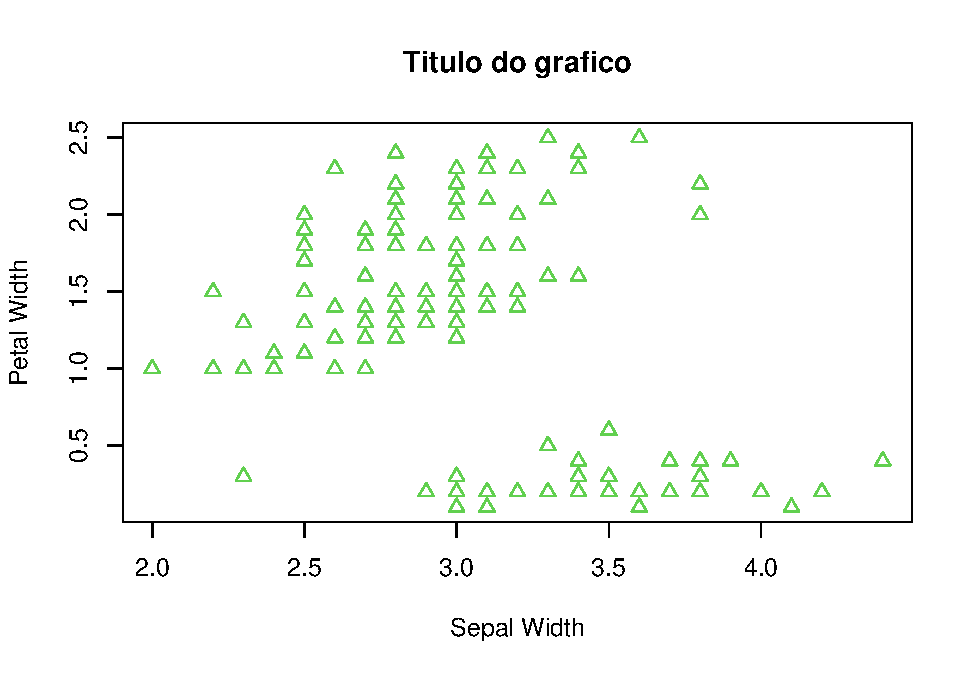
\includegraphics{_main_files/figure-latex/nome-do-chunk2-6.pdf}
\caption{\label{fig:nome-do-chunk2-6}Gráficos com R base}
\end{figure}

\hypertarget{grafico-boxplot}{%
\subsection{Grafico boxplot}\label{grafico-boxplot}}

Para criar o grafico de boxplot, iremos utilizar a variavel numerica Sepal.Width do banco de dados iris em relacao a variavel Species. Note que na funcao plot, as duas variaveis (argumentos) eram separados por virgula, aqui utilizamos o \textbf{\textasciitilde{}} para relacionar a variavel numerica com a categorica.

\begin{Shaded}
\begin{Highlighting}[]
\CommentTok{\#Importa o banco de dados iris}
\FunctionTok{data}\NormalTok{(iris)}

\CommentTok{\#Cria o grafico de boxplot basico}
\FunctionTok{boxplot}\NormalTok{(iris}\SpecialCharTok{$}\NormalTok{Sepal.Width }\SpecialCharTok{\textasciitilde{}}\NormalTok{ iris}\SpecialCharTok{$}\NormalTok{Species)}
\end{Highlighting}
\end{Shaded}

\begin{figure}
\centering
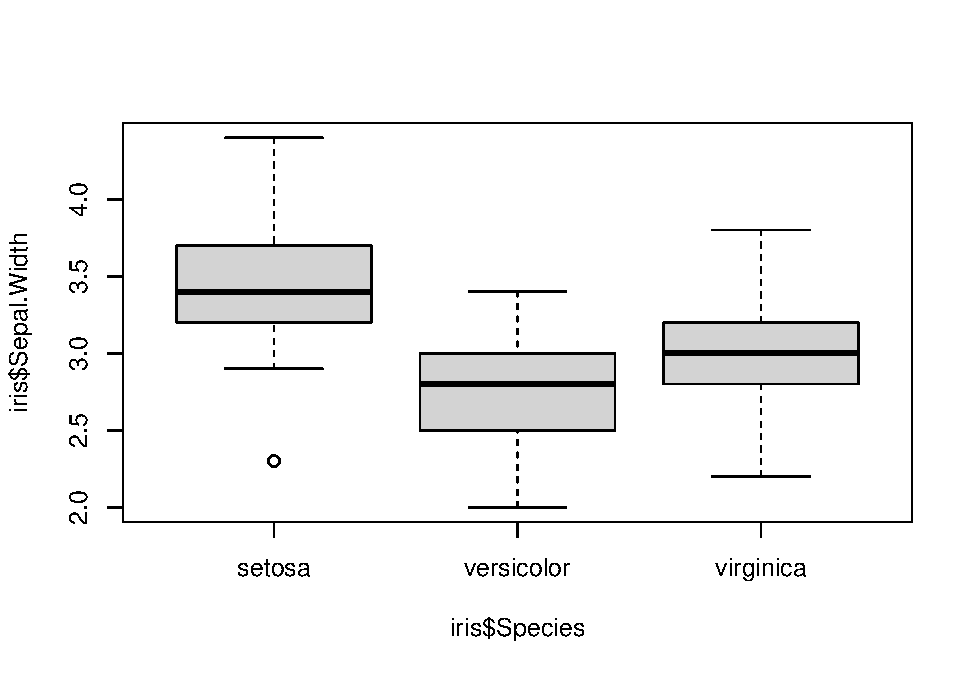
\includegraphics{_main_files/figure-latex/3_basic_boxplot-1.pdf}
\caption{(\#fig:3\_basic\_boxplot-1)Boxplot com R base utilizando o banco de dados iris}
\end{figure}

\begin{Shaded}
\begin{Highlighting}[]
\CommentTok{\#Boxplot personalizado}
\FunctionTok{boxplot}\NormalTok{(iris}\SpecialCharTok{$}\NormalTok{Sepal.Width }\SpecialCharTok{\textasciitilde{}}\NormalTok{ iris}\SpecialCharTok{$}\NormalTok{Species,}
      \AttributeTok{ylab =} \StringTok{"Petal Width"}\NormalTok{, }
      \AttributeTok{xlab =} \StringTok{"Species"}\NormalTok{,}
      \AttributeTok{col =} \FunctionTok{c}\NormalTok{(}\DecValTok{3}\NormalTok{,}\DecValTok{4}\NormalTok{,}\StringTok{"tomato"}\NormalTok{),}
      \AttributeTok{main =} \StringTok{"Titulo do grafico"}
\NormalTok{      )}
\end{Highlighting}
\end{Shaded}

\begin{figure}
\centering
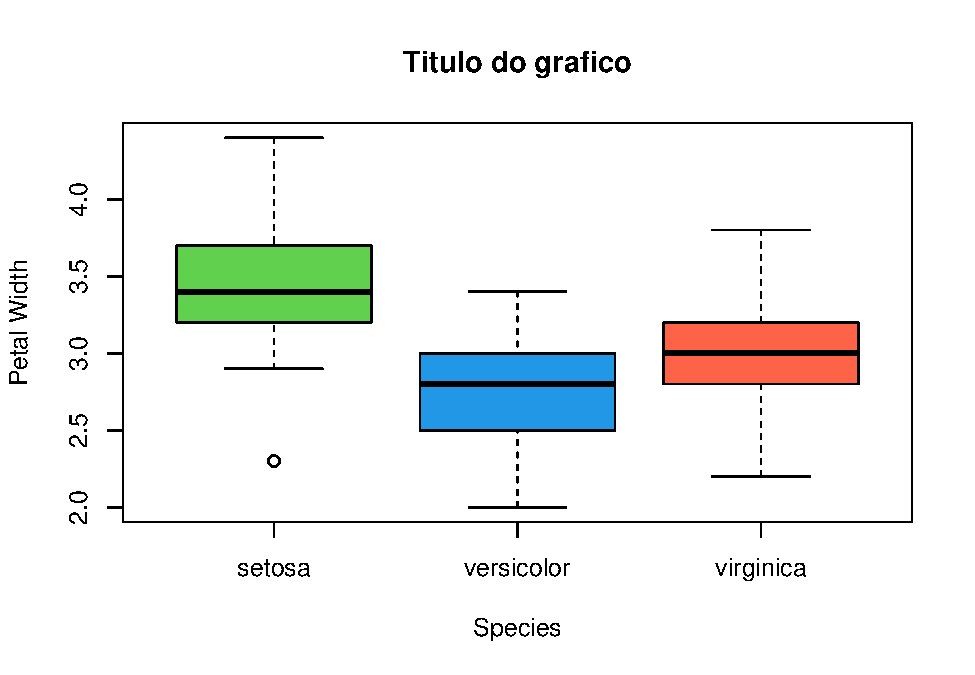
\includegraphics{_main_files/figure-latex/3_basic_boxplot-2.pdf}
\caption{(\#fig:3\_basic\_boxplot-2)Boxplot com R base utilizando o banco de dados iris}
\end{figure}

Perceba que o argumento col pode ser um vetor, e pode receber mais de um valor. Nesse caso, demos uma cor para cada fator de Species. Tente substituir os numeros por outros, ou colocar o nome das principais cores como: red, green, blue, yellow\ldots{} So nao esqueca de colocar entre aspas.

\hypertarget{grafico-de-barras}{%
\subsection{Grafico de barras}\label{grafico-de-barras}}

Para criar um grafico de barras de contagem, vamos criar nosso proprio data frame. Imagine que queremos tabular a contagem total de ectoparasitas (piolho) de ave de cada parte corporal. Como eh algo simples, podemos criar direto no R.

\begin{Shaded}
\begin{Highlighting}[]
\CommentTok{\#Criando quantidade total de parasitas}
\NormalTok{qt\_parasita }\OtherTok{\textless{}{-}} \FunctionTok{c}\NormalTok{(}\DecValTok{10}\NormalTok{, }\DecValTok{15}\NormalTok{, }\DecValTok{29}\NormalTok{, }\DecValTok{4}\NormalTok{)}

\CommentTok{\#Criando parte corporal da ave}
\NormalTok{parte\_corporal }\OtherTok{\textless{}{-}} \FunctionTok{c}\NormalTok{(}\StringTok{"cabeca"}\NormalTok{, }\StringTok{"asa"}\NormalTok{, }\StringTok{"barriga"}\NormalTok{, }\StringTok{"cauda"}\NormalTok{)}

\CommentTok{\#Criando tabela}
\NormalTok{dados\_parasita }\OtherTok{\textless{}{-}} \FunctionTok{data.frame}\NormalTok{(qt\_parasita, parte\_corporal)}

\CommentTok{\# Cria ndo gráfico de barras}
\NormalTok{grafico }\OtherTok{\textless{}{-}} \FunctionTok{barplot}\NormalTok{(dados\_parasita}\SpecialCharTok{$}\NormalTok{qt\_parasita, }
                   \AttributeTok{names.arg =}\NormalTok{ dados\_parasita}\SpecialCharTok{$}\NormalTok{parte\_corporal,}
                   \AttributeTok{xlab =} \StringTok{"Parte do Corpo"}\NormalTok{,}
                   \AttributeTok{ylab =} \StringTok{"Quantidade de Parasitas"}\NormalTok{,}
                   \AttributeTok{ylim =} \FunctionTok{c}\NormalTok{(}\DecValTok{0}\NormalTok{,}\DecValTok{35}\NormalTok{), }\CommentTok{\#define o limite do eixo y (de 0 a 35)}
                   \AttributeTok{col =} \StringTok{"lightgreen"}\NormalTok{,}
                   \AttributeTok{border =} \StringTok{"black"}\NormalTok{)}

\CommentTok{\# Adicionando os números acima das barras}
\FunctionTok{text}\NormalTok{(grafico, dados\_parasita}\SpecialCharTok{$}\NormalTok{qt\_parasita, }
\AttributeTok{labels =}\NormalTok{ dados\_parasita}\SpecialCharTok{$}\NormalTok{qt\_parasita, }\AttributeTok{pos =} \DecValTok{3}\NormalTok{, }\AttributeTok{cex =} \FloatTok{0.8}\NormalTok{)}
\end{Highlighting}
\end{Shaded}

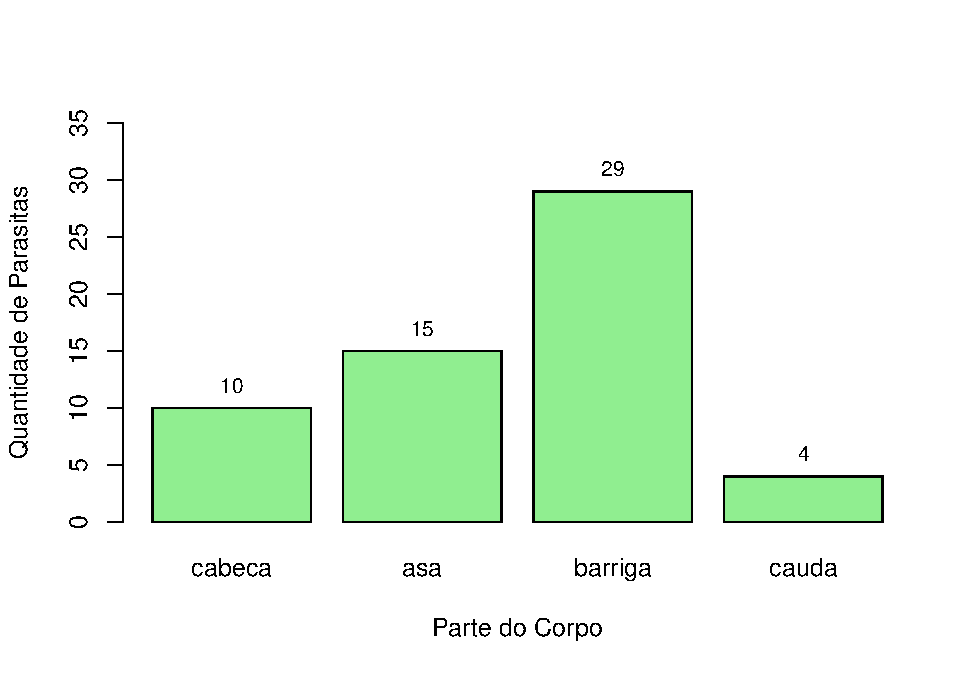
\includegraphics{_main_files/figure-latex/4_basic_hist-1.pdf}
Faca as seguintes modificacoes no codigo e veja o que acontece:

\begin{itemize}
\tightlist
\item
  Veja o que acontece se voce deletar a linha completa do argumento names.arg.\\
\item
  Troque o valor 35 de ylim por 50.\\
\item
  No argumento border, troque ``black'' por ``red'' e depois ``white''.\\
\item
  Na funcao text(), troque pos = 3, por pos = 1.\\
  (rode o grafico antes para nao sobrepor os numeros)
\end{itemize}

Eh possivel fazer muitos outros tipos de graficos, utilizando diferentes funcoes. Mas a ideia desse capitulo eh ensinar a utilizar o R, e nao a criar graficos. Entao vamos com calma, pois quando voce pensar que nao, ja foi.

\hypertarget{pacotes}{%
\section{Pacotes}\label{pacotes}}

Agora ja podemos comecar a expandir nosso universo do R. Tudo que fizemos ate agora foi utilizando o proprio R base. A partir de agora, iremos incluir um conjunto de novas funcoes atraves dos pacotes de R.
Antes de tudo, precisamos instalar o pacote que queremos utilizar, e para isso existe duas formas:

\begin{itemize}
\tightlist
\item
  Utilizando o botao \emph{Tools} do RStudio.\\
\item
  Utilizando a funcao \emph{install.packages(``nome\_do\_pacote'')}
\end{itemize}

Vamos instalar o pacote ``lattice'' para criarmos uns graficos diferentes do que fizemos anteriormente.

Utilizando o botao \emph{Tools} do RStudio click em: \textbf{Tools \textgreater{} Install package \textgreater{} digite o nome ``lattice''.} Ao comecar a digitar o R ira sugerir opcoes de pacotes com as iniciais que voce digitou. Depois clica em ``instalar''.

Utilizando a funcao \emph{install.packages()}

\begin{Shaded}
\begin{Highlighting}[]
\FunctionTok{install.packages}\NormalTok{(}\StringTok{"lattice"}\NormalTok{)}
\end{Highlighting}
\end{Shaded}

O processo de instalacao mostra no console varios processos e enquanto isso acontece, um icone de ``stop'' vermelho aparece na parte superior direita da janela do console. O processo so termina quando esse icone some e um aviso aparece:

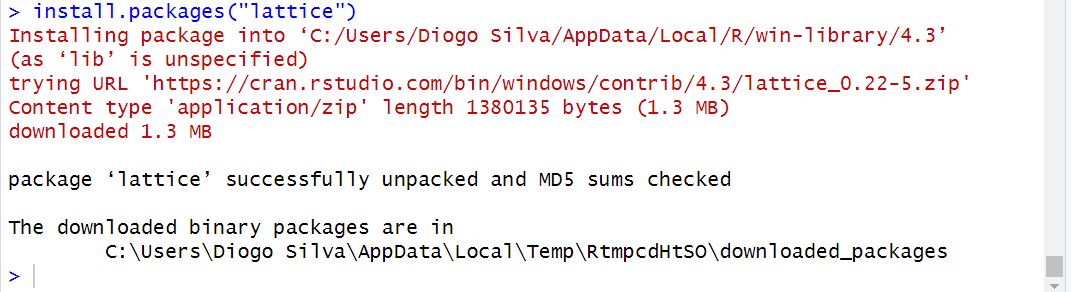
\includegraphics{img/install_package.png}

Pacote instalado, agora eh so dizer que queremos utilizar o pacote. O processo de instalacao em um determinado computador so precisa ser feito uma vez. Porem, toda vez, voce precisa dizer para o R, qual pacote voce estar utilizando. Para isso utilizamos a funcao \emph{library()}.

\begin{Shaded}
\begin{Highlighting}[]
\CommentTok{\#Carregando o pacote lattice}
\FunctionTok{library}\NormalTok{(lattice)}
\end{Highlighting}
\end{Shaded}

Se voce carregou o pacote e o R nao te retornou nenhum erro, ta tudo certo. As vezes ele te retorna um Warning message, tambem esta tudo certo. Vamos adiante.

O pacote lattice que acabamos de instalar nos fornece varias funcoes para criacao de graficos. Tenha em mente que existem milhares de pacotes cada um trazendo um conjunto de funcoes e banco de dados de diferentes contextos, tanto para criar graficos, quanto para realizar modelos estatisticos avancados.

Vamos criar alguns graficos utilizando as funcoes que o pacote lattice nos forneceu.

\begin{Shaded}
\begin{Highlighting}[]
\CommentTok{\#Se o pacote já estiver instalado, você só precisa carregar o pacote}
\FunctionTok{library}\NormalTok{(lattice) }
\end{Highlighting}
\end{Shaded}

\begin{verbatim}
## Warning: package 'lattice' was built under R version 4.3.2
\end{verbatim}

\begin{Shaded}
\begin{Highlighting}[]
\CommentTok{\# Gráfico de dispersão condicionado por uma variável}
\FunctionTok{xyplot}\NormalTok{(Sepal.Length }\SpecialCharTok{\textasciitilde{}}\NormalTok{ Sepal.Width }\SpecialCharTok{|}\NormalTok{ Species, }\AttributeTok{data =}\NormalTok{ iris,}
       \AttributeTok{main =} \StringTok{"Scatterplot Condicionado por Espécie"}\NormalTok{,}
       \AttributeTok{xlab =} \StringTok{"Largura da Sépala"}\NormalTok{, }
       \AttributeTok{ylab =} \StringTok{"Comprimento da Sépala"}\NormalTok{)}
\end{Highlighting}
\end{Shaded}

\begin{figure}
\centering
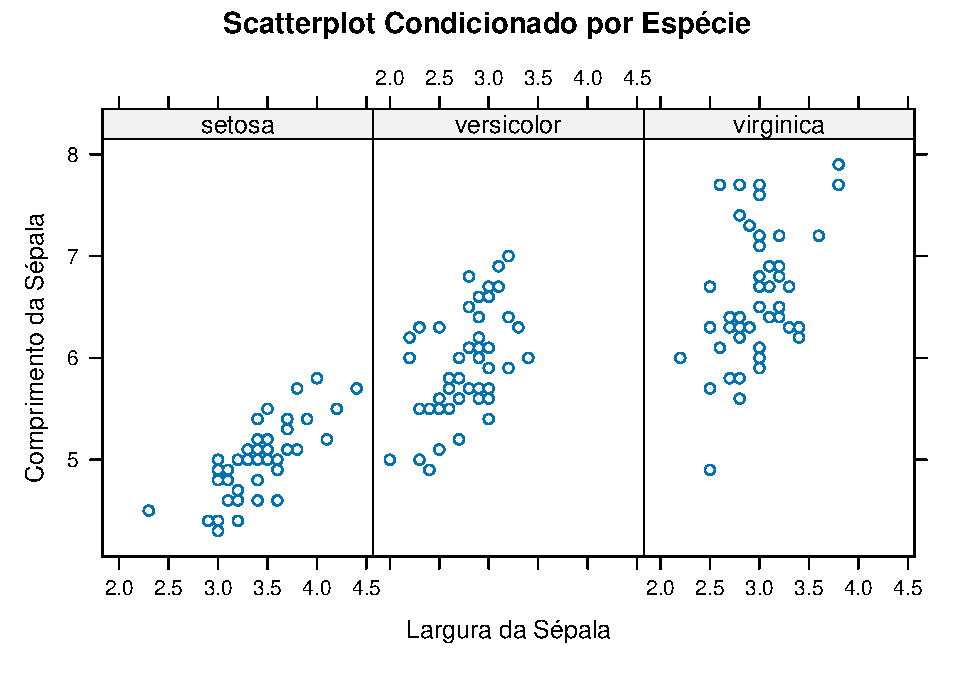
\includegraphics{_main_files/figure-latex/nome-do-chunk-1.pdf}
\caption{\label{fig:nome-do-chunk-1}Gráficos com Lattice}
\end{figure}

\begin{Shaded}
\begin{Highlighting}[]
\CommentTok{\# Histograma condicionado por uma variável}
\FunctionTok{histogram}\NormalTok{(}\SpecialCharTok{\textasciitilde{}}\NormalTok{ Petal.Length }\SpecialCharTok{|}\NormalTok{ Species, }\AttributeTok{data =}\NormalTok{ iris,}
          \AttributeTok{main =} \StringTok{"Histograma Condicionado por Espécie"}\NormalTok{,}
          \AttributeTok{xlab =} \StringTok{"Comprimento da Pétala"}\NormalTok{)}
\end{Highlighting}
\end{Shaded}

\begin{figure}
\centering
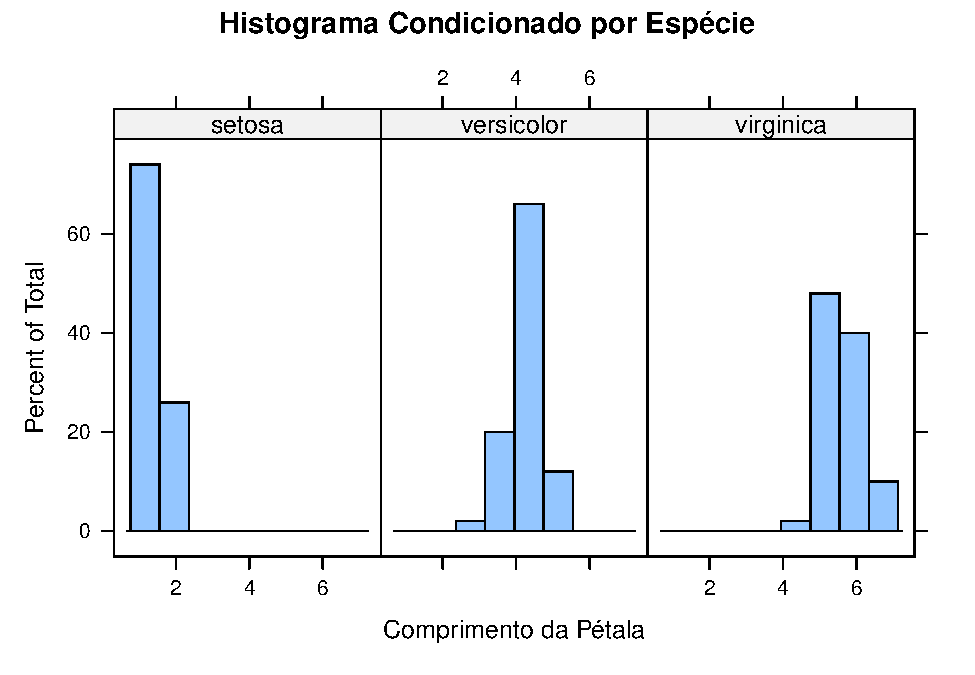
\includegraphics{_main_files/figure-latex/nome-do-chunk-2.pdf}
\caption{\label{fig:nome-do-chunk-2}Gráficos com Lattice}
\end{figure}

Acho que ja deu pra entender como o R funciona ne? Nos proximos capitulos, voce vai aprender a como trabalhar de forma eficiente no R, seguindo um fluxo de trabalho eficiente, e o melhor de tudo, reproduzivel.

\hypertarget{como-trabalhar-no-r}{%
\chapter{Como trabalhar no R}\label{como-trabalhar-no-r}}

Se voce ja tem uma nocao de R, mas ainda sente dificuldade de organizar seu fluxo de trabalho, esse capitulo eh pra voce! Utilizaremos tecnicas de ciencia de dados e repositorios como o github para tornar o trabalho no R prazeroso e eficiente!

Se voce possuir um banco de dados para analizar a quantidade de parasitas de aves da mata atlantica, ou o comportamento sexual de caranguejos chama-mares (ou seja la qual for o seu estudo), aproveite para utiliza-lo aqui nesse capitulo. Caso voce ainda nao possua seu banco de dados, trabalharemos com algum banco de dados nativo do R. Optei por utilizar o banco de dados ``iris'', mas sinta-se a vontade para utilizar qualquer outro.

Primeiro vamos exportar o banco de dados iris para que possamos simular todo o precesso desde a sua importacao. Para isso, iremos carregar o banco de dados iris utilizando a funcao \emph{data()}, e utilizaremos a funcao \emph{write.csv()} para exportar, no formato csv, a planilha ``iris'' para o computador. Deixe essa planilha salva em algum lugar no computador e finja que ela eh sua, mais para frente iremos utiliza-la.

\begin{Shaded}
\begin{Highlighting}[]

\CommentTok{\#Carregando pacote de dados iris}
\FunctionTok{data}\NormalTok{(iris)}

\CommentTok{\#Salvando (exportando) iris no computador}
\FunctionTok{write.csv}\NormalTok{(}\AttributeTok{x =}\NormalTok{ iris,            }\CommentTok{\#nome do banco de dados do R}
          \AttributeTok{file =} \StringTok{"iris.csv"}\NormalTok{,   }\CommentTok{\#nome do banco de dados salvo no computador}
          \AttributeTok{row.names =} \ConstantTok{FALSE}\NormalTok{)   }\CommentTok{\#Mostrar o nome das linhas na planilha salva utilizando TRUE ou nao utilizando FALSE.}
\end{Highlighting}
\end{Shaded}

Para entender a funcao \emph{write.csv()} modifique alguns argumentos:

\begin{itemize}
\tightlist
\item
  Substitua: file = ``iris.csv'' por file = ``planilha\_do\_R.csv''.
\item
  Substitua: row.names = FALSE, por row.names = TRUE.
\end{itemize}

Por padrao, iremos utilizar sempre row.names = FALSE.

\hypertarget{criando-um-projeto-de-r}{%
\section{Criando um projeto de R}\label{criando-um-projeto-de-r}}

Imaginemos que precisamos analisar um banco de dados de algum projeto. O primeiro passo eh criar um projeto de R, para isso voce vai no canto superior direito do RStudio (proximo a janela de environment e history) e clica :

\textbf{project (none)'' \textgreater{} new project \textgreater{} new directory \textgreater{} new project}

Ao clicar em new project, ira aparecer uma janela para escolher o nome do projeto e o local no computador que seu projeto ira ficar. Coloque o nome desejado (sugestao: ``projeto\_caranguejo''), selecione qualquer pasta no computador (sugestao: desktop) e clique em ``criar projeto''.

Se voce fez tudo direitinho, o RStudio estara do seguinte forma. Note que ao inves de project (none), estara o nome do projeto que voce criou.

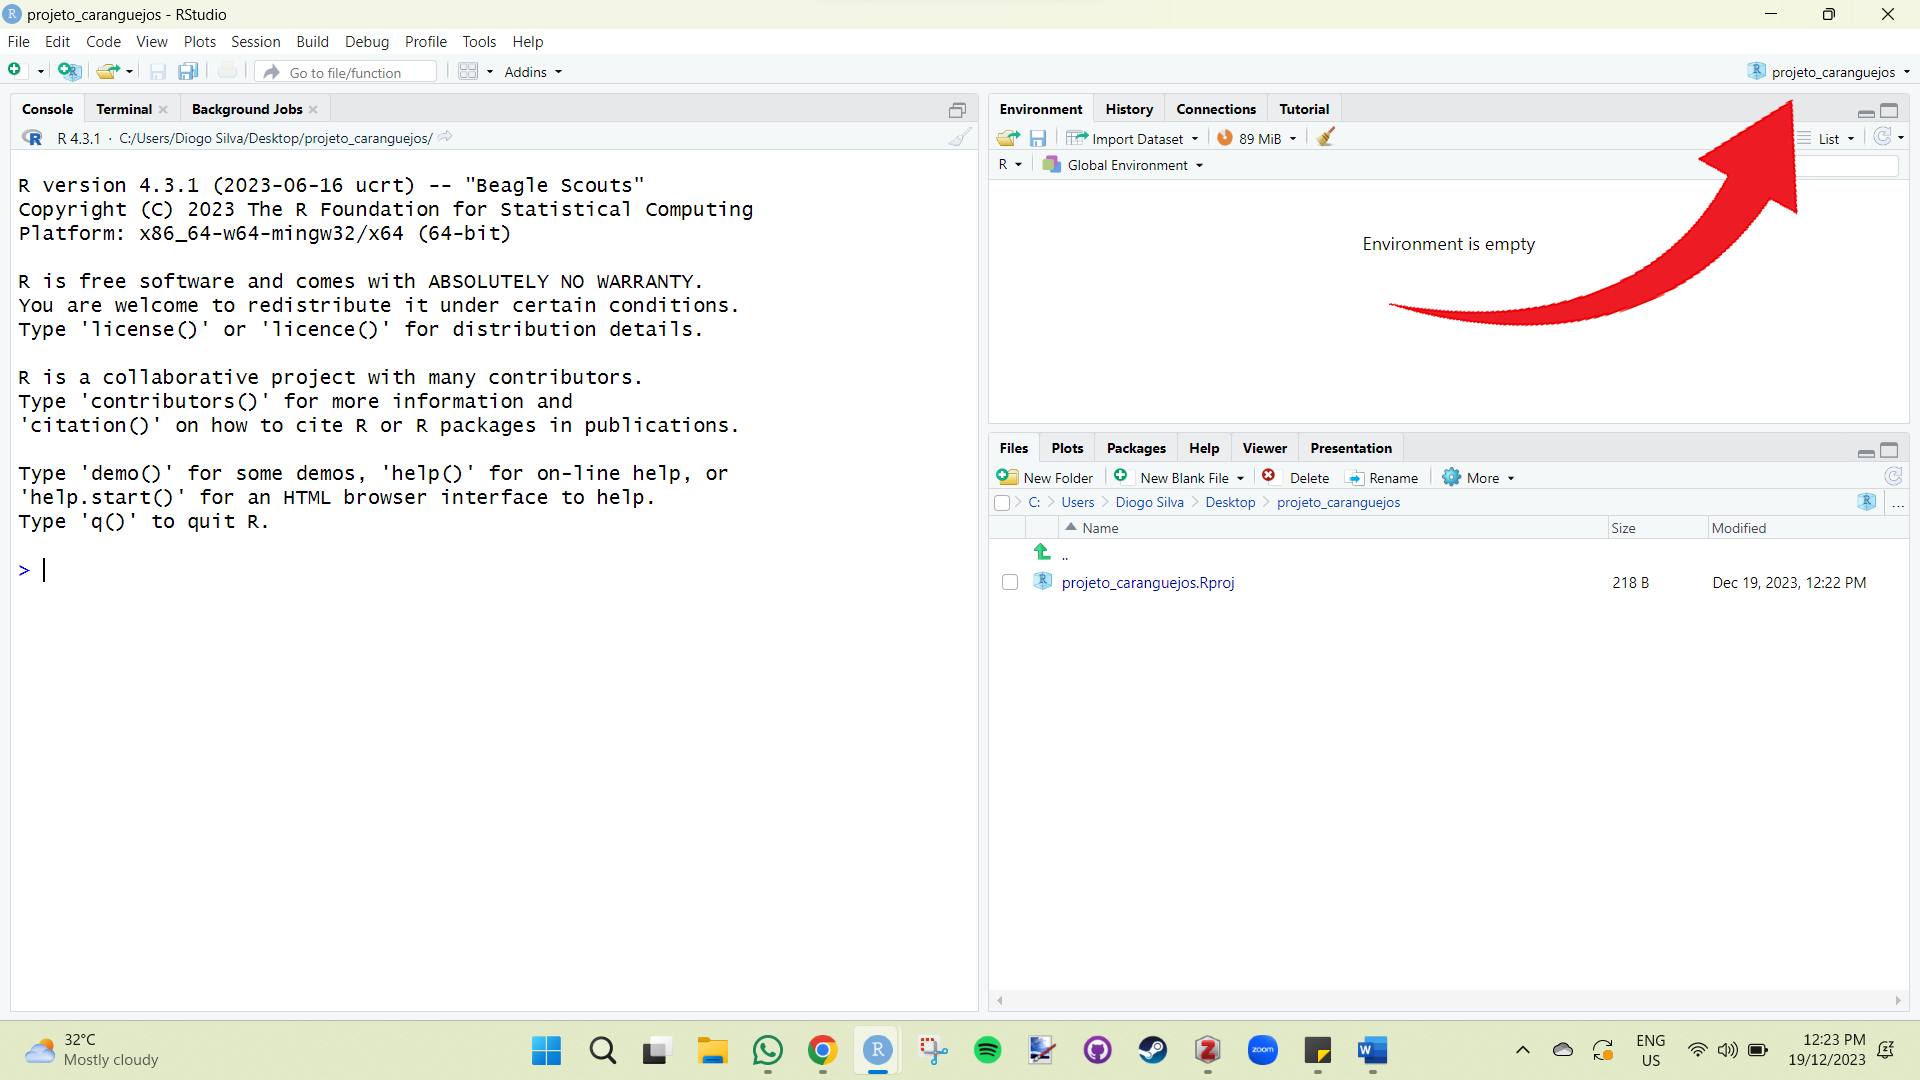
\includegraphics{img/tela_do_projeto.png}

Sugiro meu nobre consagrado leitor, que voce va no local do computador que voce criou o projeto e veja a pasta, veja o arquivo de R que foi criado. Voce tambem pode fazer isso utilizando a janela de Files, onde mostrara todas as pastas do seu diretorio que, a partir de agora, sera a pasta que o seu arquivo de projeto de R esta situado. Todos os scripts, arquivos e planilhas que voce ira utilizar nas suas analises, ficara dentro da pasta do projeto. Isso significa que vai ficar tudo solto, baguncado? Claro que nao. Iremos criar pastas organizadas onde hospedara cada coisa que iremos trabalhar como por exemplo: dados brutos, dados processados, scripts, outputs, etc. Voce pode criar manualmente, mas porque fariamos isso se temos o R para fazer por nos?

\hypertarget{organizando-o-projeto-de-r}{%
\section{Organizando o projeto de R}\label{organizando-o-projeto-de-r}}

Para criar as pastas de forma organizada, voce pode fazer manualmente ou utilizando o pacote ``here''.

\begin{Shaded}
\begin{Highlighting}[]
\FunctionTok{install.packages}\NormalTok{(}\StringTok{"here"}\NormalTok{)}
\FunctionTok{library}\NormalTok{(here)}
\end{Highlighting}
\end{Shaded}

Apos a instalacao do pacote ``here'' iremos criar uma funcao que criara as pastas automaticamente no nosso diretorio. Nao se assuste com o script da funcao, ela eh mais simples do que parece e voce nao precisa entende-lo por completo. Apenas rode o codigo para criar a funcao e depois rode o codigo que utiliza a funcao para criar as pastas.

Antes de rodar o codigo, certifique-se de que voce esta no projeto de R que voce criou.

\begin{Shaded}
\begin{Highlighting}[]
\CommentTok{\# Criando funcao para criacao das pastas do projeto}
\NormalTok{build\_project }\OtherTok{\textless{}{-}} \ControlFlowTok{function}\NormalTok{(}\AttributeTok{type =} \StringTok{"analysis"}\NormalTok{,}
                          \AttributeTok{temp =} \ConstantTok{TRUE}\NormalTok{) \{}
  
  \ControlFlowTok{if}\NormalTok{(type }\SpecialCharTok{==} \StringTok{"analysis"}\NormalTok{)\{}
    \CommentTok{\# Data}
    \FunctionTok{dir.create}\NormalTok{(}\AttributeTok{path =}\NormalTok{ here}\SpecialCharTok{::}\FunctionTok{here}\NormalTok{(}\StringTok{"data"}\NormalTok{))}
    \FunctionTok{dir.create}\NormalTok{(}\AttributeTok{path =}\NormalTok{ here}\SpecialCharTok{::}\FunctionTok{here}\NormalTok{(}\StringTok{"data"}\NormalTok{, }\StringTok{"raw"}\NormalTok{))}
    \FunctionTok{dir.create}\NormalTok{(}\AttributeTok{path =}\NormalTok{ here}\SpecialCharTok{::}\FunctionTok{here}\NormalTok{(}\StringTok{"data"}\NormalTok{, }\StringTok{"processed"}\NormalTok{))}
    
    \CommentTok{\# outputs}
    \FunctionTok{dir.create}\NormalTok{(}\AttributeTok{path =}\NormalTok{ here}\SpecialCharTok{::}\FunctionTok{here}\NormalTok{(}\StringTok{"outputs"}\NormalTok{))}
    \FunctionTok{dir.create}\NormalTok{(}\AttributeTok{path =}\NormalTok{ here}\SpecialCharTok{::}\FunctionTok{here}\NormalTok{(}\StringTok{"outputs"}\NormalTok{, }\StringTok{"figures"}\NormalTok{))}
    \FunctionTok{dir.create}\NormalTok{(}\AttributeTok{path =}\NormalTok{ here}\SpecialCharTok{::}\FunctionTok{here}\NormalTok{(}\StringTok{"outputs"}\NormalTok{, }\StringTok{"tables"}\NormalTok{))}
    \ControlFlowTok{if}\NormalTok{(}\FunctionTok{isTRUE}\NormalTok{(temp))\{}
      \FunctionTok{dir.create}\NormalTok{(}\AttributeTok{path =}\NormalTok{ here}\SpecialCharTok{::}\FunctionTok{here}\NormalTok{(}\StringTok{"outputs"}\NormalTok{, }\StringTok{"temp"}\NormalTok{))}
\NormalTok{    \}}
    
    \CommentTok{\# scripts}
    \FunctionTok{dir.create}\NormalTok{(}\AttributeTok{path =}\NormalTok{ here}\SpecialCharTok{::}\FunctionTok{here}\NormalTok{(}\StringTok{"scripts"}\NormalTok{))}
    
    \CommentTok{\# docs}
    \CommentTok{\#dir.create(path = here::here("docs")) \#para criar a pasta docs, so tirar o comentario dessa linha}
\NormalTok{  \}}
\NormalTok{\}}

\CommentTok{\#Utilizando a funcao criada para gerar as pastas}
\FunctionTok{build\_project}\NormalTok{(}\AttributeTok{type =} \StringTok{"analysis"}\NormalTok{,}
              \AttributeTok{temp =} \ConstantTok{TRUE}\NormalTok{) }\CommentTok{\#se FALSE, nao cria a pasta temp.}
\end{Highlighting}
\end{Shaded}

Se tudo ocorreu bem, as pastas estao assim:

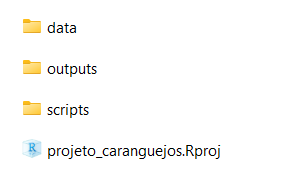
\includegraphics{img/pastas_do_projeto.png}

Dentro da pasta data voce encontra as pastas ``raw'' e ``processed''. Em outputs voce encontra ``figures'', ``temp'' e ``tables''. Em script, voce encontrara nada (por enquanto). O arquivo com o simbolo do R ``projeto\_caranguejos.Rproj'' eh o seu projeto de R. Voce pode abri-lo (dando duplo clique) toda vez que voce for trabalhar no projeto. Isso abrira o Rstudio ja com o seu projeto aberto e pronto para trabalhar.

\begin{itemize}
\tightlist
\item
  Feche o RStudio e abra-o novamente dando clique duplo no seu projeto de R.
\end{itemize}

Agora voce tem tudo pronto para comecar a trabalhar com um fluxo de trabalho eficiente e reprodutivel!

\hypertarget{trabalhando-em-um-projeto-de-r}{%
\section{Trabalhando em um projeto de R}\label{trabalhando-em-um-projeto-de-r}}

Antes de tudo baixe a planilha de dados ficticios de uma especie de passarinho (tambem ficticia), que contem informacoes ficticias sobre peso (g) e quantidade de parasitas de tres diferentes localidades (A, B, C):

\href{data/fake_data.xlsx}{Clique aqui para baixar a planilha ficticia}

Na pasta \textbf{data \textgreater{} raw} voce adiciona sua planilha de dados brutos ficticias (fake\_data.xlsx). O fluxo de trabalho sera o mais simples possivel, mas envolvera etapas essenciais da analise de dados.

\textbf{Limpar dados brutos \textgreater{} Realizar analise \textgreater{} Mostrar graficos}

Para limpar a planilha de dados brutos, iremos criar um script para isso. Utilizaremos funcoes do pacote dplyr para modificar nome das variaveis, nome dos fatores, analisar dados faltantes, entre outras coisas.

\hypertarget{etapa-1-limpar-dados}{%
\subsection{Etapa 1: limpar dados}\label{etapa-1-limpar-dados}}

Vamos criar um script para limpar nossos dados brutos. Monte o script completo utilizando os codigos que irei fornecendo a seguir copiando e colando no seu RStudio. Assim, a primeira coisa que iremos fazer do script eh seu cabecalho. Utilizaremos os comentarios para criar um cabecalho com as informacoes de titulo, autores e data.

\begin{Shaded}
\begin{Highlighting}[]

\CommentTok{\# Script to load and clean raw data flores iris}
\CommentTok{\# Author: Marilia T. Ericcson}
\CommentTok{\# Data: 2019{-}11{-}06}
\end{Highlighting}
\end{Shaded}

Apos isso, utilizaremos os comentarios, para organizar o script em topicos fazendo manualmente ou utilizando o atalho: \textbf{ctrl + shift + R}. A primeira parte do codigo eh a instalacao dos pacotes que iremos utilizar no processo.

\begin{Shaded}
\begin{Highlighting}[]

\CommentTok{\# Packages {-}{-}{-}{-}{-}{-}{-}{-}{-}{-}{-}{-}{-}{-}{-}{-}{-}{-}{-}{-}{-}{-}{-}{-}{-}{-}{-}{-}{-}{-}{-}{-}{-}{-}{-}{-}{-}{-}{-}{-}{-}{-}{-}{-}{-}{-}{-}{-}{-}{-}{-}{-}{-}{-}{-}{-}{-}{-}{-}{-}{-}}
\ControlFlowTok{if}\NormalTok{(}\SpecialCharTok{!}\FunctionTok{require}\NormalTok{(dplyr)) }\FunctionTok{install.packages}\NormalTok{(}\StringTok{"dplyr"}\NormalTok{) }\CommentTok{\#se o pacote dplyr nao estiver sido instalado, ele sera instalado.}
\FunctionTok{library}\NormalTok{(dplyr) }\CommentTok{\#carregar pacote}
\end{Highlighting}
\end{Shaded}

Segundo, importamos o banco de dados a ser processado (limpado) utilizando a funcao \emph{read.csv()} e atribuindo (\textless-) a um objeto que iremos chamar de ``dados''. Para importar voce so precisa especificar o caminho do diretorio em que o arquivo ta inserido. Como estamos utilizando o projeto de R, o diretorio eh onde o projeto esta. Dessa forma, nao ha necessidade de dizer para o R qual o seu diretorio de trabalho. Logo fica facil importar os dados brutos pois sabemos que ele esta na pasta dados \textgreater{} raw \textgreater{} iris.csv. Dizemos isso para o R utilizando os nomes das pastas separado por barras e por fim, o nome do arquivo (iris) e suas extensao (.csv).

\begin{Shaded}
\begin{Highlighting}[]

\CommentTok{\# Load data {-}{-}{-}{-}{-}{-}{-}{-}{-}{-}{-}{-}{-}{-}{-}{-}{-}{-}{-}{-}{-}{-}{-}{-}{-}{-}{-}{-}{-}{-}{-}{-}{-}{-}{-}{-}{-}{-}{-}{-}{-}{-}{-}{-}{-}{-}{-}{-}{-}{-}{-}{-}{-}{-}{-}{-}{-}{-}{-}{-}{-}{-}{-}}
\NormalTok{dados }\OtherTok{\textless{}{-}} \FunctionTok{read.csv}\NormalTok{(}\StringTok{"data/raw/iris.csv"}\NormalTok{)}
\end{Highlighting}
\end{Shaded}

Agora que o banco de dados foi importado, podemos fazer um check up basico utilizando algumas funcoes.

\begin{Shaded}
\begin{Highlighting}[]

\CommentTok{\# 1. Basic checks {-}{-}{-}{-}{-}{-}{-}{-}{-}{-}{-}{-}{-}{-}{-}{-}{-}{-}{-}{-}{-}{-}{-}{-}{-}{-}{-}{-}{-}{-}{-}{-}{-}{-}{-}{-}{-}{-}{-}{-}{-}{-}{-}{-}{-}{-}{-}{-}{-}{-}{-}{-}{-}{-}{-}{-}{-}{-}{-}{-}{-}{-}}
\FunctionTok{nrow}\NormalTok{(dados)             }\CommentTok{\# How many rows}
\FunctionTok{str}\NormalTok{(dados)              }\CommentTok{\# Variables classes}
\FunctionTok{attributes}\NormalTok{(dados)       }\CommentTok{\# Attributres}
\FunctionTok{head}\NormalTok{(dados)             }\CommentTok{\# First rows}
\FunctionTok{any}\NormalTok{(}\FunctionTok{duplicated}\NormalTok{(dados))  }\CommentTok{\# There is any duplicated rows?}
\FunctionTok{any}\NormalTok{(}\FunctionTok{is.na}\NormalTok{(dados))       }\CommentTok{\# There are NAs in the data?}
\end{Highlighting}
\end{Shaded}

As vezes os nomes das variaveis nao sao faceis de trabalhar, possuindo espaco, acentos, letras maiusculas e minusculas, e nomes confusos. Alem de complicar o codigo, o nome de algumas variaveis podem bugar o script (caso das acentuacoes de palavras em portugues). Entao vamos mudar o nome das variaveis utilizando a funcao \emph{rename()} do pacote \textbf{dplyr}. Iremos deixar os nomes mais faceis de trabalhar, deixando todas as letras minusculas.

\begin{Shaded}
\begin{Highlighting}[]

\CommentTok{\# 3. Rename columns names{-}{-}{-}{-}{-}{-}{-}{-}{-}{-}{-}{-}{-}{-}{-}{-}{-}{-}{-}{-}{-}{-}{-}{-}{-}{-}{-}{-}{-}{-}{-}{-}{-}{-}{-}{-}{-}{-}{-}{-}{-}{-}{-}{-}{-}{-}{-}{-}{-}{-}{-}{-}{-}{-}{-}}
\FunctionTok{head}\NormalTok{(dados)}
\NormalTok{dados2 }\OtherTok{\textless{}{-}} \FunctionTok{rename}\NormalTok{(iris,                         }\CommentTok{\#sua planilha bruta}
                 \AttributeTok{sepal\_length =}\NormalTok{ Sepal.Length,  }\CommentTok{\#nomes das variaveis (nome\_novo = nome antigo)}
                 \AttributeTok{sepal\_width  =}\NormalTok{ Sepal.Width,}
                 \AttributeTok{petal\_length =}\NormalTok{ Petal.Length,}
                 \AttributeTok{petal\_width  =}\NormalTok{ Petal.Width,}
                 \AttributeTok{species      =}\NormalTok{ Species)}
\FunctionTok{head}\NormalTok{(dados2)}
\end{Highlighting}
\end{Shaded}

Agora vamos dizer para o R os tipos de nossas variaveis. Um problema muito comum, eh o R nao reconhecer que a variavel categorica, nao possui fatores, mesmo possuindo. Por exemplo, em ``iris'', temos a variavel categorica `Species' com seus fatores (setosa, versicolor, virginica). Eh possivel que no seu banco de dados, o R nao reconheca isso, entao vamos utilizar a funcao \emph{levels()} para verificar se o R entendeu quais sao os fatores. Se o R retornar NULL, voce precisa dizer para o R utilizando a funcao \emph{as.factor()}.

\begin{Shaded}
\begin{Highlighting}[]

\CommentTok{\# 4. Fix factor variables{-}{-}{-}{-}{-}{-}{-}{-}{-}{-}{-}{-}{-}{-}{-}{-}{-}{-}{-}{-}{-}{-}{-}{-}{-}{-}{-}{-}{-}{-}{-}{-}{-}{-}{-}{-}{-}{-}{-}{-}{-}{-}{-}{-}{-}{-}{-}{-}{-}{-}{-}{-}{-}{-}{-}}
\CommentTok{\# check factor variable}
\FunctionTok{levels}\NormalTok{(dados2}\SpecialCharTok{$}\NormalTok{species)}

\CommentTok{\# making factor variables}
\NormalTok{dados2}\SpecialCharTok{$}\NormalTok{species }\OtherTok{\textless{}{-}} \FunctionTok{as.factor}\NormalTok{(dados2}\SpecialCharTok{$}\NormalTok{species) }\CommentTok{\#atribuindo a variavel specie transformada a ela mesma.}

\CommentTok{\# check factor variable}
\FunctionTok{levels}\NormalTok{(dados2}\SpecialCharTok{$}\NormalTok{species)}
\end{Highlighting}
\end{Shaded}

Agora podemos renomear o nome dos fatores de uma variavel categorica utilizando a funcao \emph{recode\_factor()}. Nesse processo podemos identificar erros de digitacao que ocorreram durante o planilhamento dos dados. Por exemplo, voce pode ter digitado ``Macho'', ``macho'' e ``male'' na variavel sexo durante o planilhamento. O R vai identificar os tres como sendo fatores diferentes mas na verdade sao o mesmo fator. Portanto eh necessario que seja padronizado.

\begin{Shaded}
\begin{Highlighting}[]
\CommentTok{\# 4.1 fix species factors}

\CommentTok{\#check factors}
\FunctionTok{levels}\NormalTok{(dados2}\SpecialCharTok{$}\NormalTok{species)}

\CommentTok{\#rename factors}
\NormalTok{dados2}\SpecialCharTok{$}\NormalTok{species }\OtherTok{\textless{}{-}} \FunctionTok{recode\_factor}\NormalTok{(dados2}\SpecialCharTok{$}\NormalTok{species,                 }\CommentTok{\#variavel categorica}
                                \AttributeTok{setosa =} \StringTok{"iris\_setosa"}\NormalTok{,         }\CommentTok{\#mudando nome setosa para iris\_setosa}
                                \AttributeTok{versicolor =} \StringTok{"iris\_versicolor"}\NormalTok{,}
                                \AttributeTok{virginica =} \StringTok{"iris\_virginica"}\NormalTok{)}

\CommentTok{\#check factors}
\FunctionTok{levels}\NormalTok{(dados2}\SpecialCharTok{$}\NormalTok{species)}
\end{Highlighting}
\end{Shaded}

Agora que limpamos nossos dados brutos, iremos exportar nossa planilha limpa. Perceba que o processo do script eh colocar a planilha bruta de um lado e sair limpa e bonitinha do outro. Eh com os dados processados que iremos trabalhar de fato. Vamos salvar sempre no formato csv por ser um formato mais simples, leve e estavel.

\begin{Shaded}
\begin{Highlighting}[]
\CommentTok{\# 8. Save processed data {-}{-}{-}{-}{-}{-}{-}{-}{-}{-}{-}{-}{-}{-}{-}{-}{-}{-}{-}{-}{-}{-}{-}{-}{-}{-}{-}{-}{-}{-}{-}{-}{-}{-}{-}{-}{-}{-}{-}{-}{-}{-}{-}{-}{-}{-}{-}{-}{-}{-}{-}{-}{-}}
\FunctionTok{write.csv}\NormalTok{(}\AttributeTok{x =}\NormalTok{ dados2,                                 }\CommentTok{\#nome da planilha que voce quer exportar}
          \AttributeTok{file =} \StringTok{"data/processed/processed\_iris.csv"}\NormalTok{, }\CommentTok{\#local e nome da planilha exportada}
          \AttributeTok{row.names =} \ConstantTok{FALSE}\NormalTok{)                          }\CommentTok{\#sempre utilizaremos row.names = FALSE}
\end{Highlighting}
\end{Shaded}

O processo de manipulacao de dados no R eh bastante completo e existem diferentes formas de limpar seus dados brutos. O pacote \textbf{dplyr} possui funcoes capazes de selecionar variaveis, selecionar linhas, criar variaveis, criar subsets, entre outras. Para aprimorar seu script de limpeza de dados, voce precisara aprender sobre manipulacao de dados e incluir no processo, os codigos no seu script. Por sorte, existe muito material disponivel na internet sobre o assunto. Talvez algum dia eu crie um material sobre manipulacao de dados com dplyr, mas aqui esse nao eh meu objetivo. Meu objetivo eh simplesmente fornecer o esqueleto teorico, te dando base para crescer de forma mais direcionada.

Por fim, nao esqueca de salvar o script na pasta script com o nome `01\_clean\_raw\_data'.

\hypertarget{etapa-2-fazer-analise}{%
\subsection{Etapa 2: fazer analise}\label{etapa-2-fazer-analise}}

Com a planilha bruta processada, podemos realizar testes estatisticos para responder nossa hipotese. Vamos supor que nossa pergunta seja saber se existe diferenca entre o tamanho das petalas entre as tres especies. Organizaremos o script de analise de forma similar ao script de limpeza, ou seja, escreveremos um cabecalho, carregaremos pacotes, importaremos e analisaremos dados de forma organizada.

Vamos fazer um cabecalho para nosso script de analise.

\begin{Shaded}
\begin{Highlighting}[]

\CommentTok{\# Script to load and analyse processed data iris}
\CommentTok{\# Author: Marilia T. Ericcson}
\CommentTok{\# Data: 2019{-}11{-}07}
\end{Highlighting}
\end{Shaded}

Vamos criar o codigo para carregar os pacotes que iremos utilizar

\begin{Shaded}
\begin{Highlighting}[]

\CommentTok{\#Carregar pacotes}
\FunctionTok{library}\NormalTok{(broom)}
\end{Highlighting}
\end{Shaded}

Dessa vez iremos importar a planilha limpa e processada. Note que o caminho de importacao eh similar ao caminho que exportamos no script de limpeza.

\begin{Shaded}
\begin{Highlighting}[]

\CommentTok{\# Load data {-}{-}{-}{-}{-}{-}{-}{-}{-}{-}{-}{-}{-}{-}{-}{-}{-}{-}{-}{-}{-}{-}{-}{-}{-}{-}{-}{-}{-}{-}{-}{-}{-}{-}{-}{-}{-}{-}{-}{-}{-}{-}{-}{-}{-}{-}{-}{-}{-}{-}{-}{-}{-}{-}{-}{-}{-}{-}{-}{-}{-}{-}{-}}
\NormalTok{dados }\OtherTok{\textless{}{-}} \FunctionTok{read.csv}\NormalTok{(}\StringTok{"data/processed/processed\_iris.csv"}\NormalTok{)}
\end{Highlighting}
\end{Shaded}

Vamos fazer um check basico.

\begin{Shaded}
\begin{Highlighting}[]

\CommentTok{\# 1. Basic checks {-}{-}{-}{-}{-}{-}{-}{-}{-}{-}{-}{-}{-}{-}{-}{-}{-}{-}{-}{-}{-}{-}{-}{-}{-}{-}{-}{-}{-}{-}{-}{-}{-}{-}{-}{-}{-}{-}{-}{-}{-}{-}{-}{-}{-}{-}{-}{-}{-}{-}{-}{-}{-}{-}{-}{-}{-}{-}{-}{-}{-}{-}}
\FunctionTok{head}\NormalTok{(dados)}
\FunctionTok{str}\NormalTok{(dados)}
\FunctionTok{leves}\NormalTok{(dados}\SpecialCharTok{$}\NormalTok{species)}
\end{Highlighting}
\end{Shaded}

Vamos realizar uma analise para comparar a largura das petalas entre as especies. Para isso, iremos utilizar o teste nao parametrico de kruskal-wallis atraves da funcao kruskal.test(). Nessa funcao, voce precisa dizer qual sua variavel numerica de interesse em relacao a (\textasciitilde) sua variavel categorica e seus grupos (fatores). Veja que o p-value eh menor que 0.05, entao dizemos que existe diferenca da largura entre as tres especies.

\begin{Shaded}
\begin{Highlighting}[]

\CommentTok{\#realizando o teste}
\NormalTok{kw }\OtherTok{\textless{}{-}} \FunctionTok{kruskal.test}\NormalTok{(iris}\SpecialCharTok{$}\NormalTok{Sepal.Width }\SpecialCharTok{\textasciitilde{}}\NormalTok{ iris}\SpecialCharTok{$}\NormalTok{Species)}
\NormalTok{kw}
\end{Highlighting}
\end{Shaded}

Vamos salvar o resultado em uma tabela organizada (tidy) utilizando a funcao \emph{tidy()} do pacote \textbf{broom}.

\begin{Shaded}
\begin{Highlighting}[]

\CommentTok{\#Ajeitando tabela para formato tidy}
\NormalTok{table\_kw }\OtherTok{\textless{}{-}} \FunctionTok{tidy}\NormalTok{(kw\_test)}
\NormalTok{table\_kw}
\end{Highlighting}
\end{Shaded}

Agora salvaremos essa tabela na nossa pasta outputs em tables.

\begin{Shaded}
\begin{Highlighting}[]

\CommentTok{\#Exportando resultado}
\FunctionTok{write.csv}\NormalTok{(}\AttributeTok{x =}\NormalTok{ table\_kw,                                 }
          \AttributeTok{file =} \StringTok{"outputs/tables/resultado\_kw.csv"}\NormalTok{,}
          \AttributeTok{row.names =} \ConstantTok{FALSE}\NormalTok{)}
\end{Highlighting}
\end{Shaded}

Maravilha! Ja temos nosso segundo script pronto. Agora eh so salva-lo na pasta script com o nome: `02\_kruskal\_test'.

\hypertarget{etapa-3-criar-grafico}{%
\subsection{Etapa 3: criar grafico}\label{etapa-3-criar-grafico}}

Agora vamos criar o grafico para representar nosso resultado de que existe diferenca da largura das petadas entre as especies de iris.

\begin{Shaded}
\begin{Highlighting}[]
 
\CommentTok{\# Script to load and analyse processed data iris}
\CommentTok{\# Author: Marilia T. Ericcson}
\CommentTok{\# Data: 2019{-}11{-}07}
 
\CommentTok{\#Carregar pacotes}
\FunctionTok{library}\NormalTok{(ggplot2)}

\CommentTok{\# Load data {-}{-}{-}{-}{-}{-}{-}{-}{-}{-}{-}{-}{-}{-}{-}{-}{-}{-}{-}{-}{-}{-}{-}{-}{-}{-}{-}{-}{-}{-}{-}{-}{-}{-}{-}{-}{-}{-}{-}{-}{-}{-}{-}{-}{-}{-}{-}{-}{-}{-}{-}{-}{-}{-}{-}{-}{-}{-}{-}{-}{-}{-}{-}}
\NormalTok{dados }\OtherTok{\textless{}{-}} \FunctionTok{read.csv}\NormalTok{(}\StringTok{"data/processed/processed\_iris.csv"}\NormalTok{)}

\CommentTok{\# 1. Basic checks {-}{-}{-}{-}{-}{-}{-}{-}{-}{-}{-}{-}{-}{-}{-}{-}{-}{-}{-}{-}{-}{-}{-}{-}{-}{-}{-}{-}{-}{-}{-}{-}{-}{-}{-}{-}{-}{-}{-}{-}{-}{-}{-}{-}{-}{-}{-}{-}{-}{-}{-}{-}{-}{-}{-}{-}{-}{-}{-}{-}{-}{-}}
\FunctionTok{head}\NormalTok{(dados)}
\FunctionTok{str}\NormalTok{(dados)}
\FunctionTok{leves}\NormalTok{(dados}\SpecialCharTok{$}\NormalTok{species)}

\CommentTok{\# 2. Criar grafico boxplot {-}{-}{-}{-}{-}{-}{-}{-}{-}{-}{-}{-}{-}{-}{-}{-}{-}{-}{-}{-}{-}{-}{-}{-}{-}{-}{-}{-}{-}{-}{-}{-}{-}{-}{-}{-}{-}{-}{-}{-}{-}{-}{-}{-}{-}{-}{-}{-}{-}{-}{-}{-}{-}}

\NormalTok{grafico }\OtherTok{\textless{}{-}} \FunctionTok{ggplot}\NormalTok{(dados, }\FunctionTok{aes}\NormalTok{(}\AttributeTok{x =}\NormalTok{ species, }\AttributeTok{y =}\NormalTok{ petal\_width))}\SpecialCharTok{+}
  \FunctionTok{geom\_boxplot}\NormalTok{()}

\NormalTok{grafico}

\CommentTok{\# 3. Salvando grafico {-}{-}{-}{-}{-}{-}{-}{-}{-}{-}{-}{-}{-}{-}{-}{-}{-}{-}{-}{-}{-}{-}{-}{-}{-}{-}{-}{-}{-}{-}{-}{-}{-}{-}{-}{-}{-}{-}{-}{-}{-}{-}{-}{-}{-}{-}{-}{-}{-}{-}{-}{-}{-}{-}{-}{-}{-}{-}}

\FunctionTok{ggsave}\NormalTok{(}\AttributeTok{plot =}\NormalTok{ grafico,    }\CommentTok{\#nome do grafico}
       \AttributeTok{filename =} \StringTok{"output/figures/Grafico\_boxplot.png"}\NormalTok{, }\CommentTok{\#nome do grafico exportado}
       \AttributeTok{width =} \DecValTok{10}\NormalTok{,                             }\CommentTok{\#largura do grafico}
       \AttributeTok{height =} \DecValTok{10}\NormalTok{,                            }\CommentTok{\#Altura do grafico}
       \AttributeTok{dpi =} \DecValTok{300}\NormalTok{)                              }\CommentTok{\#resolucao do grafico}
\end{Highlighting}
\end{Shaded}

\begin{figure}
\centering
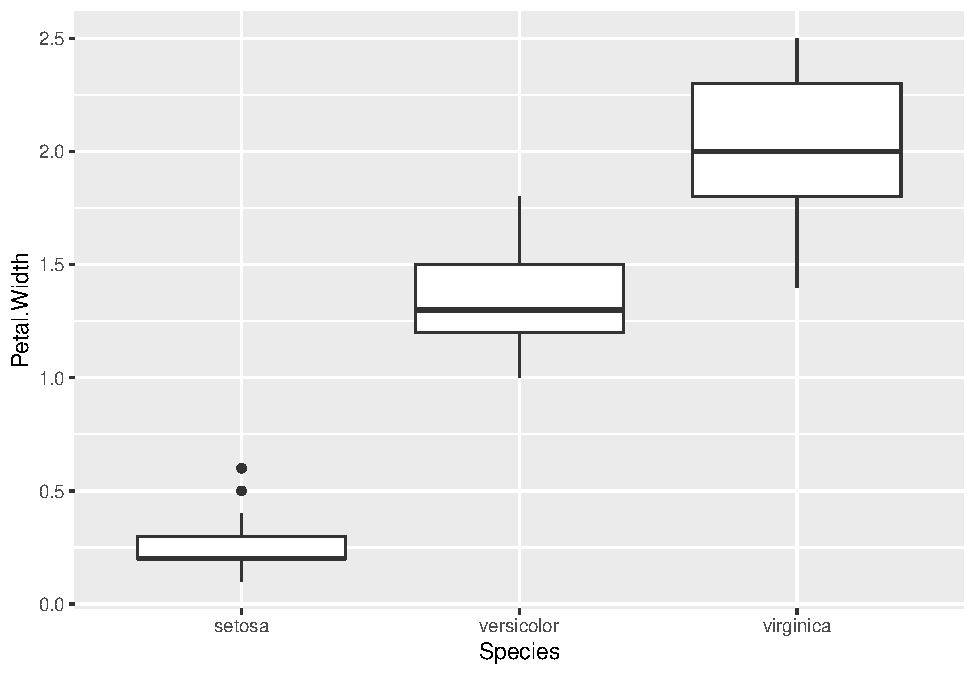
\includegraphics{_main_files/figure-latex/graph-1.pdf}
\caption{\label{fig:graph}ggplot2}
\end{figure}

Voce acabou de criar um grafico utilizando o pacote ggplot2 que eh o pacote mais utilizado para producao de graficos no R. O codigo pode parecer um pouco confuso no inicio, mas nao precisa estudar muito para perceber que ele eh muito simples e intuitivo. Para aprender mais sobre graficos, sugiro os livros: \url{https://rkabacoff.github.io/datavis/} e \url{https://r-graphics.org/}

Nao esqueca de salvar o script com o nome `03\_grafico'
\#Etapa 4: Replicabilidade

O seu projeto esta organizado de forma que se torna facil a replicabilidade em qualquer computador gerando todos seus outputs (tabelas e figuras) automaticamente! Para isso, voce precisa manter e JAMAIS deletar ou modificar seus dados brutos (pasta raw). Todos os demais arquivos podem ser produzidos com um click a partir dos seus dados brutos, portanto, podem ser deletados. Isso se torna util ao compartilhar seus dados com alguem, em que voce pode zipar todo seu projeto, enviar para um contribuidor e ele podera ter acesso a tudo rodando apenas um script. Eh esse script que iremos fazer agora.

\begin{Shaded}
\begin{Highlighting}[]
\CommentTok{\# Script to run all project code}
\CommentTok{\# Importante: reinicie o R antes de rodar esse script session \textgreater{} restart R}

\CommentTok{\# Start{-}{-}{-}{-}}
\CommentTok{\# 1. Run all scripts again on a fresh R section{-}{-}{-}{-}{-}{-}{-}{-}{-}{-}{-}{-}{-}{-}{-}{-}{-}{-}{-}{-}{-}{-}{-}{-}{-}{-}{-}{-}{-}{-}{-}{-}{-}}
\CommentTok{\# 1.1 Load and clean data{-}{-}{-}{-}}
\FunctionTok{source}\NormalTok{(}\AttributeTok{file =} \StringTok{"script/01\_clean\_raw\_data.R"}\NormalTok{)}

\CommentTok{\# 1.2 Run analysis {-}{-}{-}{-}{-}{-}{-}{-}{-}{-}{-}{-}{-}{-}{-}{-}{-}{-}{-}{-}{-}{-}{-}{-}{-}{-}{-}{-}{-}{-}{-}{-}{-}{-}{-}{-}{-}{-}{-}{-}{-}{-}{-}{-}{-}{-}{-}{-}{-}{-}{-}{-}{-}{-}{-}{-}{-}{-}{-}{-}{-}}
\FunctionTok{source}\NormalTok{(}\AttributeTok{file =} \StringTok{"script/02\_kruskal\_test.R"}\NormalTok{)}

\CommentTok{\# 1.3 Plot figures{-}{-}{-}{-}{-}{-}{-}{-}{-}{-}{-}{-}{-}{-}{-}{-}{-}{-}{-}{-}{-}{-}{-}{-}{-}{-}{-}{-}{-}{-}{-}{-}{-}{-}{-}{-}{-}{-}{-}{-}{-}{-}{-}{-}{-}{-}{-}{-}{-}{-}{-}{-}{-}{-}{-}{-}{-}{-}{-}{-}{-}{-}}
\FunctionTok{source}\NormalTok{(}\AttributeTok{file =} \StringTok{"script/03\_grafico.R"}\NormalTok{)}
\end{Highlighting}
\end{Shaded}

Ao rodar esse codigo, todos os seus scripts sao rodados e todos os seus outputs e planilhas processadas sao geradas. Mas lembre, seu dado bruto contido na pasta data/raw, nao pode ser deletada ou modificada.

Salve esse script com o nome ``run\_project''.

\hypertarget{git-e-github}{%
\chapter{Git e GitHub}\label{git-e-github}}

  \bibliography{book.bib}

\end{document}
